\documentclass[12pt,twosides,onecolumn,openany]{article}
\usepackage{graphicx} 


\usepackage[catalan]{babel}
\usepackage{emptypage}
\usepackage{hyperref}
\usepackage{mathtools}
\usepackage{blindtext}
\usepackage{subfigure}
\usepackage[utf8]{inputenc}
\usepackage{caption}
\usepackage{subcaption}
\usepackage{wrapfig}
\usepackage[a4paper]{geometry}
\geometry{top=2.5cm, bottom=2.5cm, left=2.5cm, right=2.5cm}
\usepackage{fancyhdr}
\pagestyle{fancy}
\usepackage{amsmath}
\usepackage{amssymb}
\usepackage{amsfonts}
\providecommand{\norm}[1]{\lVert#1\rVert}
\hypersetup{colorlinks=true,urlcolor=blue,linkcolor=blue}
\usepackage{multirow}
\usepackage{multicol}
\usepackage{rotating}

\usepackage{titlesec}

\newenvironment{Figura}
  {\par\medskip\noindent\minipage{\linewidth}}
  {\endminipage\par\medskip}

\titleformat{\section}  % comando de sección a formatear
  {\fontsize{14}{16}\bfseries} % formato para toda la línea
  {\thesection} % cómo mostrar el número
  {0.4em} % espacio entre el número y el texto
  {} % formato solo para el texto
  [] % formato para después del texto


\fancyhf{}
\fancyhead[LO,RE]{Grup D3}
\fancyhead[RO,LE]{Pràctica IIIb}
\fancyfoot[LO,RE]{\thepage}
\fancyfoot[RO,LE]{Laboratori de Termodinàmica - UAB}
\graphicspath{ {images/} }

\begin{document}

\begin{center}
    {\Large \textsc{Gasos reals: Isotermes d'Andrews - Estudi del punt crític}}\\
    \vspace{0.2cm}
    \textsc{3 d'Octubre de 2024}\\
    \vspace{0.2cm}
    Miguel A. - 1637738
\end{center}
\begin{center}
    \textsc{\textit{RESUM}}
\end{center}
En aquesta pràctica es fa un estudi del comportament de l'hexafluorur de sofre (SF$_6$) a prop del seu punt crític. A partir de mesures de pressió i volum en condicions isotèrmiques del SF$_6$ en estat gasós, s'observa el comportament al llarg de la seva transició de fase vapor-líquid. Fent servir diagrames com el de Clapeyron, d'Amagat o $pV$ vs $V^{-1}$ es realitza l'estudi del gas per a obtenir el seu punt crític experimentalment i es compara amb dades obtingudes de la literatura. Es realitza una estimació del nombre de mols del sistema estudiat i finalment es compara el seu comportament de gas real amb el comportament de gas ideal i de gas de Van der Waals.
\vspace{0.5cm}
\begin{multicols}{2}
\section{Introducció i objecctius}
L'estudi d'un gas real implica un esforç empíric considerable, en comparació amb sistemes amb comportament de gas ideal. El comportament d'un gas ideal ve condicionat per diverses suposicions que en simplifiquen l'estudi. En un gas ideal se suposa que les partícules que el componen són adimensionals i no interactuen entre elles, les considerem immutables (no reaccionen químicament) i col·lisionen elàsticament amb les parets del recipient que conté el gas.\\\\
En aquesta pràctica realitzarem l'estudi d'un gas real, l'hexafluorur de sofre (SF$_6$). S'observa que el seu comportament difereix de l'ideal, i que apareix el fenomen de la transició de fase. També es mostra com el comportament d'aquesta transició de fase ve determinat pel punt crític del gas. L'objectiu principal de l'estudi és trobar les coordenades $p$, $V$ i $T$ d'aquest punt crític.
\section{Fonament teòric}
L'equació tèrmica que descriu un gas ideal és
\begin{equation}\label{gas_ideal}
  pV = nRT
\end{equation}
on $R$ és la constant dels gasos ideals, $p$ la pressió, $V$ el volum, $T$ la temperatura i $n$ el nombre de mols del sistema. Definim el coeficient de compressió a partir de la relació
\begin{equation}\label{factor_compress}
  z = \frac{pV}{nRT}
\end{equation}
que, per a un gas ideal compleix que equival a la unitat. Amb el gas ideal com a referència, podem comparar la compressibilitat dels gasos. Si per a un gas qualsevol, aquest coeficient s'apropa més a la unitat és més compressible, si s'allunya és més incompressible.\\\\
S'observa empíricament com per a una transició de fase de primera espècie apareix una discontinuïtat en el volum molar entre les fases \cite{transicions}. Per a una transició vapor-líquid per compressió en condicions isotèrmiques, s'observa com el sistema heterogeni líquid + gas disminueix de forma contínua, i com alhora varien les fraccions molars de cada component mentre es manté la pressió constant. Anomenem a aquesta pressió de la transició com a pressió de vapor, tant l'increment de volum necessari per a realitzar la transició com la pressió de vapor són dependents de la temperatura. A més, durant una transició de fase existeix una discontinuïtat entròpica molar, fent que existeixi un intercanvi d'energia en forma de calor donat per
\begin{equation}\label{Clausius}
  \frac{\text{d}p}{\text{d}T} = n \frac{L^{\text{lv}}}{T \Delta V}
\end{equation}
on $L^{\text{lv}}$ és la calor latent de vaportizació i $\Delta V$ l'increment de volum necessari per a realitzar la transició.\\\\
Existeixen diversos models que intenten explicar el comportament d'un gas real. Entre ells tenim el model de gas real de Van der Waals
\begin{equation}\label{gas_VdW}
  \left[ p + a \left( \frac{n}{V} \right)^2\right]\left( \frac{V}{n} - b \right) = RT
\end{equation}
, obtingut de considerar un cert volum a les partícules del gas \cite{physical_chemistry}. Els coeficients $a$ i $b$ són coeficients que s'obtenen empíricament i depenen de les característiques del gas estudiat. Obtenim el seu valor a partir d'imposar les condicions de punt crític. El punt crític d'un gas és aquella tripleta de valors $p$, $T$ i $v$ a partir de la qual ja no s'observa una transició de fase\footnote{Per a temperatures més altes d'aquest punt parlem d'un fluid supercrític.}. Determinem el punt crític com el punt d'inflexió de la funció $p(V)$, i als punts on comença i acaba la transició de fase conformen el que anomenem com a corba de saturació. El màxim de la corba de saturació coincideix amb el punt crític del fluid. Derivant dos cops l'Equació \eqref{gas_VdW} i igualant a zero trobem que
\begin{equation}\label{coef_VdW}
  a = \frac{9}{8} RT_cv_c \hspace{0.4cm} , \hspace{0.6cm} b=\frac{1}{3}v_c
\end{equation}
substituïnt a l'equació de Van der Waals
\begin{equation}\label{nostre_gas_VdW}
  p = \frac{nRT}{V-V_c/3} - \frac{9}{8}RT_c \frac{nV_c}{V^2}
\end{equation}
i concretament per al punt crític d'un gas de Van der Waals es compleix que
\begin{equation}\label{critic_VdW}
  v_c = \frac{3}{8} \frac{RT_c}{p_c}
\end{equation}
Aquest model de gas real no acaba de descriure correctament les transicions de fase. Existeixen punts de les corbes de Van der Waals que incompleixen la condició d'estabilitat:
\begin{equation}\label{cond_estabilitat}
  k_{T} = -\frac{1}{V}\left( \frac{\partial V}{\partial p} \right)_{T} > 0
\end{equation}
on $k_T$ és el coeficient de compressibilitat isotèrmica.
També podem descriure un gas real a partir del desenvolupament del virial
\begin{multline}\label{virial}
  p = RT \left[ \frac{n}{V} + B(T)\left( \frac{n}{V} \right)^2 + \right.\\ \left.+ C(T) \left( \frac{n}{V} \right)^3 + \dots \right]
\end{multline}
on $B(T)$ i $C(T)$ són funcions de la temperatura característiques per a cada gas. Aprofitarem aquest desenvolupament quedant-nos només a segon ordre:
\begin{equation}\label{virial_tallat}
  pV = nRT + B(T)n^2\frac{1}{V}
\end{equation}
    
\section{Procediment experimental}
Estudiarem les propietats de l'hexafluorur de sofre (SF$_6$) en condicions isotèrmiques al voltant del punt crític. Per a fer-ho, disposem del muntatge que s'observa a la Figura \ref{fig:muntatge_experimental}.
\begin{Figura}
  \centering
  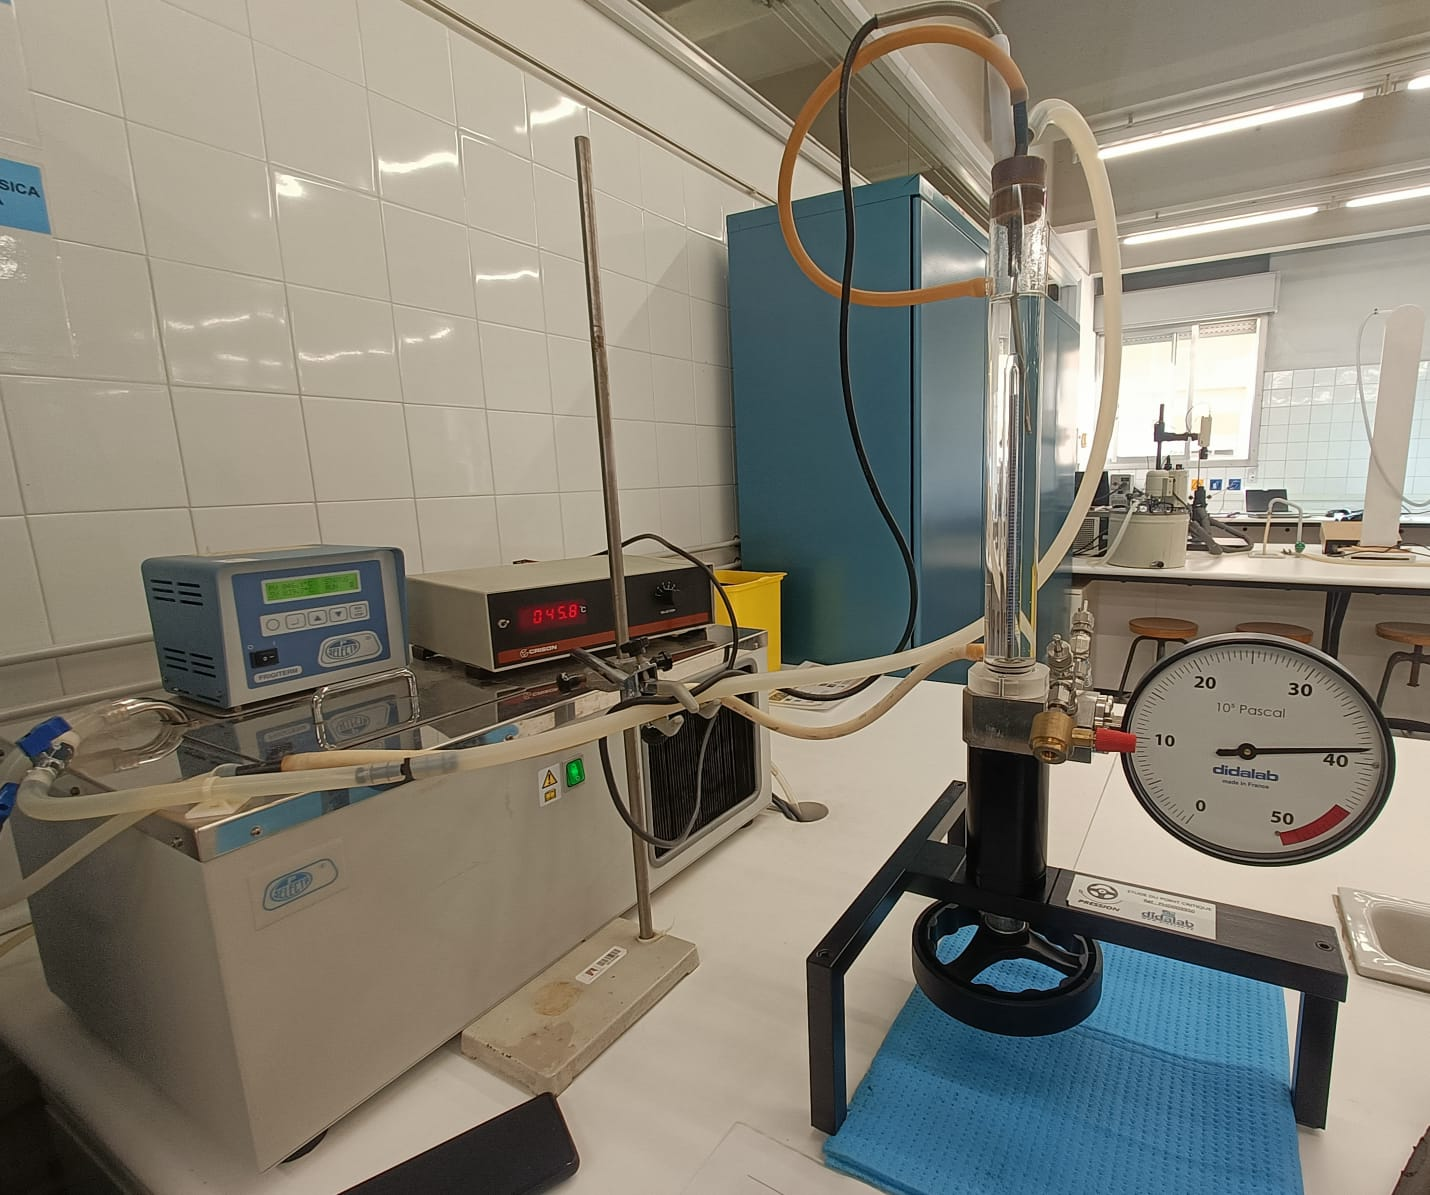
\includegraphics[width=0.85\linewidth]{../../reports/practica_IIIb/images/muntatge_experimental_IIIb.jpeg}
  \captionof{figure}{\footnotesize{Muntatge experimental de la pràctica. S'observa a la part dreta de la imatge una proveta graduada, submergida dins d'un bany tèrmic i amb una clau a la base que controla el pistó; a un costat s'observa un manòmetre i a la part superior tubs que mantenen el bany tèrmic i un termòmetre de sonda. A la part esquerra es veu el sistema que garanteix el bany tèrmic, format per un aparell que aporta calor i altra que refrigera. }}
  \label{fig:muntatge_experimental}
\end{Figura}
Aquest muntatge consta principalment d'una proveta graduada de vidre amb SF$_6$ i mercuri a l'interior, un pistó que podem moure amb una clau, un bany tèrmic, un termòmetre i un manòmetre per a realitzar les mesures. La proveta se situa dins d'un tub, també de vidre, que conté aigua a la temperatura constant desitjada (actuant com a bany tèrmic). Les parets de vidre de la proveta a l'interior són gruixudes, de forma que evita que es trenqui quan apliquem pressions elevades. Tot i això, durant la pràctica es procura no superar el llindar màxim de pressió, marcat en vermell al manòmetre a uns \(45\,\text{bar}\). Podem mesurar el volum del SF$_6$ observant qué marca el nivell de mercuri a l'interior de la proveta. El mercuri és un fluid incompressible, si reduim el volum de l'interior de la proveta fent servir el pistó només variarà el volum del SF$_6$.\\\\
Com la quantitat de mesures experimentals són considerables, es reparteix la tasca entre quatre grups de laboratori. Cada grup es dedica a mesurar els punts de pressió i volum per a dues isotermes, posteriorment es reuneix la informació per a poder realitzar l'estudi. En aquesta pràctica s'han mesurat les isotermes per a una temperatura de \(25\,^\circ\text{C}\) i altra de \(45\,^\circ\text{C}\). Per a seguir un ordre, comencem realitzant mesures per a un bany tèrmic a baixa temperatura i posteriorment a alta temperatura.\\\\
Situem un volum inicial de SF$_6$ a la proveta no superior als \(4\,\text{ml}\) per tal de no causar fuites del gas. Es realitzen mesures pujant el nivell de mercuri amb un pas de volum de \(\sim 0,2 \, \text{ml}\). Es procura que els canvis de volum siguin lents, de forma quasiestàtica, i deixem temps entre mesura i mesura per tal d'evitar estats metaestables al fluid.\\\\
A part d'aquestes mesures experimentals, també es realitza l'experiència d'observar el comportament del fluid a temperatura superior a la del punt crític, el qual s'ha estudiat només de forma qualitativa.
\section{Resultats i discussió}
Al llarg de les mesures realitzades per a cada isoterma, s'ha intentat mantenir el sistema en un bany tèrmic a temperatura constant, propera als valors objectiu. A causa de la complicació del calibratge del bany tèrmic, les isotermes no corresponen a una temperatura exacta de, per exemple, \(25\,^\circ\text{C}\) o \(45\,^\circ\text{C}\). Anotem la mesura de la temperatura del bany tèrmic a la Taula \ref{bany_tèrmic}. Observem a la mateixa taula que associem el seu valor enter desitjat com a etiqueta, a partir d'ara ens referirem a les temperatures mesurades amb la corresponent etiqueta.
\renewcommand{\arraystretch}{1.3}
\begin{Figura}
  \centering
  \captionof{table}{\footnotesize{Mesures de la temperatura amb les seves respectives etiquetes.}}
  \begin{tabular}{c|c}
    Etiqueta & $T_{\text{bany}}$ ($\pm0,1$) [$^\circ$C] \\
    \hline\hline
    10 & 10,9 \\
    15 & 15,7 \\
    20 & 20,2 \\
    25 & 25,3 \\
    30 & 30,3 \\
    35 & 35,0 \\
    40 & 40,0 \\
    45 & 44,7 \\
  \end{tabular}
  \label{bany_tèrmic}
\end{Figura}
\renewcommand{\arraystretch}{1}
En el cas particular de les isotermes realitzades pel nostre grup, s'han pressenciat els comportaments del gas al voltant del punt crític de forma qualitativa tant per a \(25 \, ^\circ\text{C}\) com per a \(45 \, ^\circ\text{C}\). Com es podrà veure més endavant al diagrama de Clapeyron o als de Van der Waals, la temperatura baixa correspon a una isoterma on es presencia un canvi de fase i la temperatura alta a una temperatura molt a prop de la temperatura crítica. A temperatura baixa era notable com el gas arribava a un punt on no variava la seva pressió i es començava a liquar. A temperatura alta, aquesta distinció del canvi de fase encara hi era, però deixà de ser tan notable. Al estar tan a prop del punt crític començava a adquirir aspecte d'un fluid supercrític.\\\\
En realitzar l'experiència a una temperatura superior a la crítica, ja no s'observaven transicions de fase. El canvi en la pressió no presentava en cap moment un comportament isobàric, augmentava de forma contínua i no s'arriba a distingir si el fluid és líquid o gas.\\\\
De forma paral·lela a realitzar les mesures de la pràctica, s'han realitzat algunes comprovacions qualitatives del comportament del fluid reaccionant a diferents estímuls. A temperatures i pressions properes al punt crític s'observava un aplanament del menisc. Això és causat perquè les densitats s'igualen a mesura que ens apropem al punt crític.\\\\
També s'ha comprovat com, en realitzar expansions febles, però ràpides, apareixen estats metaestables en forma de boira al voltant del menisc.
\subsection{Diagrama de Clapeyron}
A partir de les dades experimentals obtingudes al laboratori construïm el diagrama de Clapeyron\footnote{Representem $V$ com a $V_{\text{sist}}$ degut a que s'han realitzat mesures tant del sistema sencer (sigui en fase homogènia o heterogènia) com de només el volum que ocupa la fase vapor.} $p$ vs $V$ que s'observa a la Figura \ref{fig:Diagrama_Clapeyron}. Els punts marcats de color negre representen els punts de saturació, aquelles coordenades de volum i pressió on s'observa la liquació del SF$_6$. Atès que el procediment de mesura ha sigut realitzat per diferents grups, que el pas de volum que hi ha entre punt i punt és massa gran i a possibles errors humans a l'hora de mesurar, s'ha fet un tractament d'aquestes dades de saturació amb la motivació d'obtenir resultats més coherents.\\\\
Aquest tractament es realitza amb raonaments físics, primer de tot, s'han igualat els valors de pressió a cada parella de punts de saturació de cada isoterma a la seva pressió de vapor mesurada, d'aquesta manera fixem l'inici i final del tram conodal que s'hauria d'obtenir. Com a segon tractament, tenint en compte que potser aquests valors de pressió de vapor no corresponen als volums que marquen els punts conodals mesurats, a cada parell de mesures de saturació que, respecte al seu veïnatge, s'observi un interval de volum considerablement alt (al voltant de \(0,2\,\text{ml}\), veure Annex), se substitueix el valor mesurat per la mitjana dels dos punts consecutius. Com a tercera modificació, donat que \(T \simeq  45 \, ^{\circ}\text{C}\) és un valor al voltant de la temperatura crítica del SF$_6$, es desplacen un punt a la dreta del seu valor original de forma que coincideixin amb l'aparent punt d'inflexió que marca la corba de dades experimentals a \(\sim 45 \, ^{\circ}\text{C}\).
\begin{Figura}
  \centering
  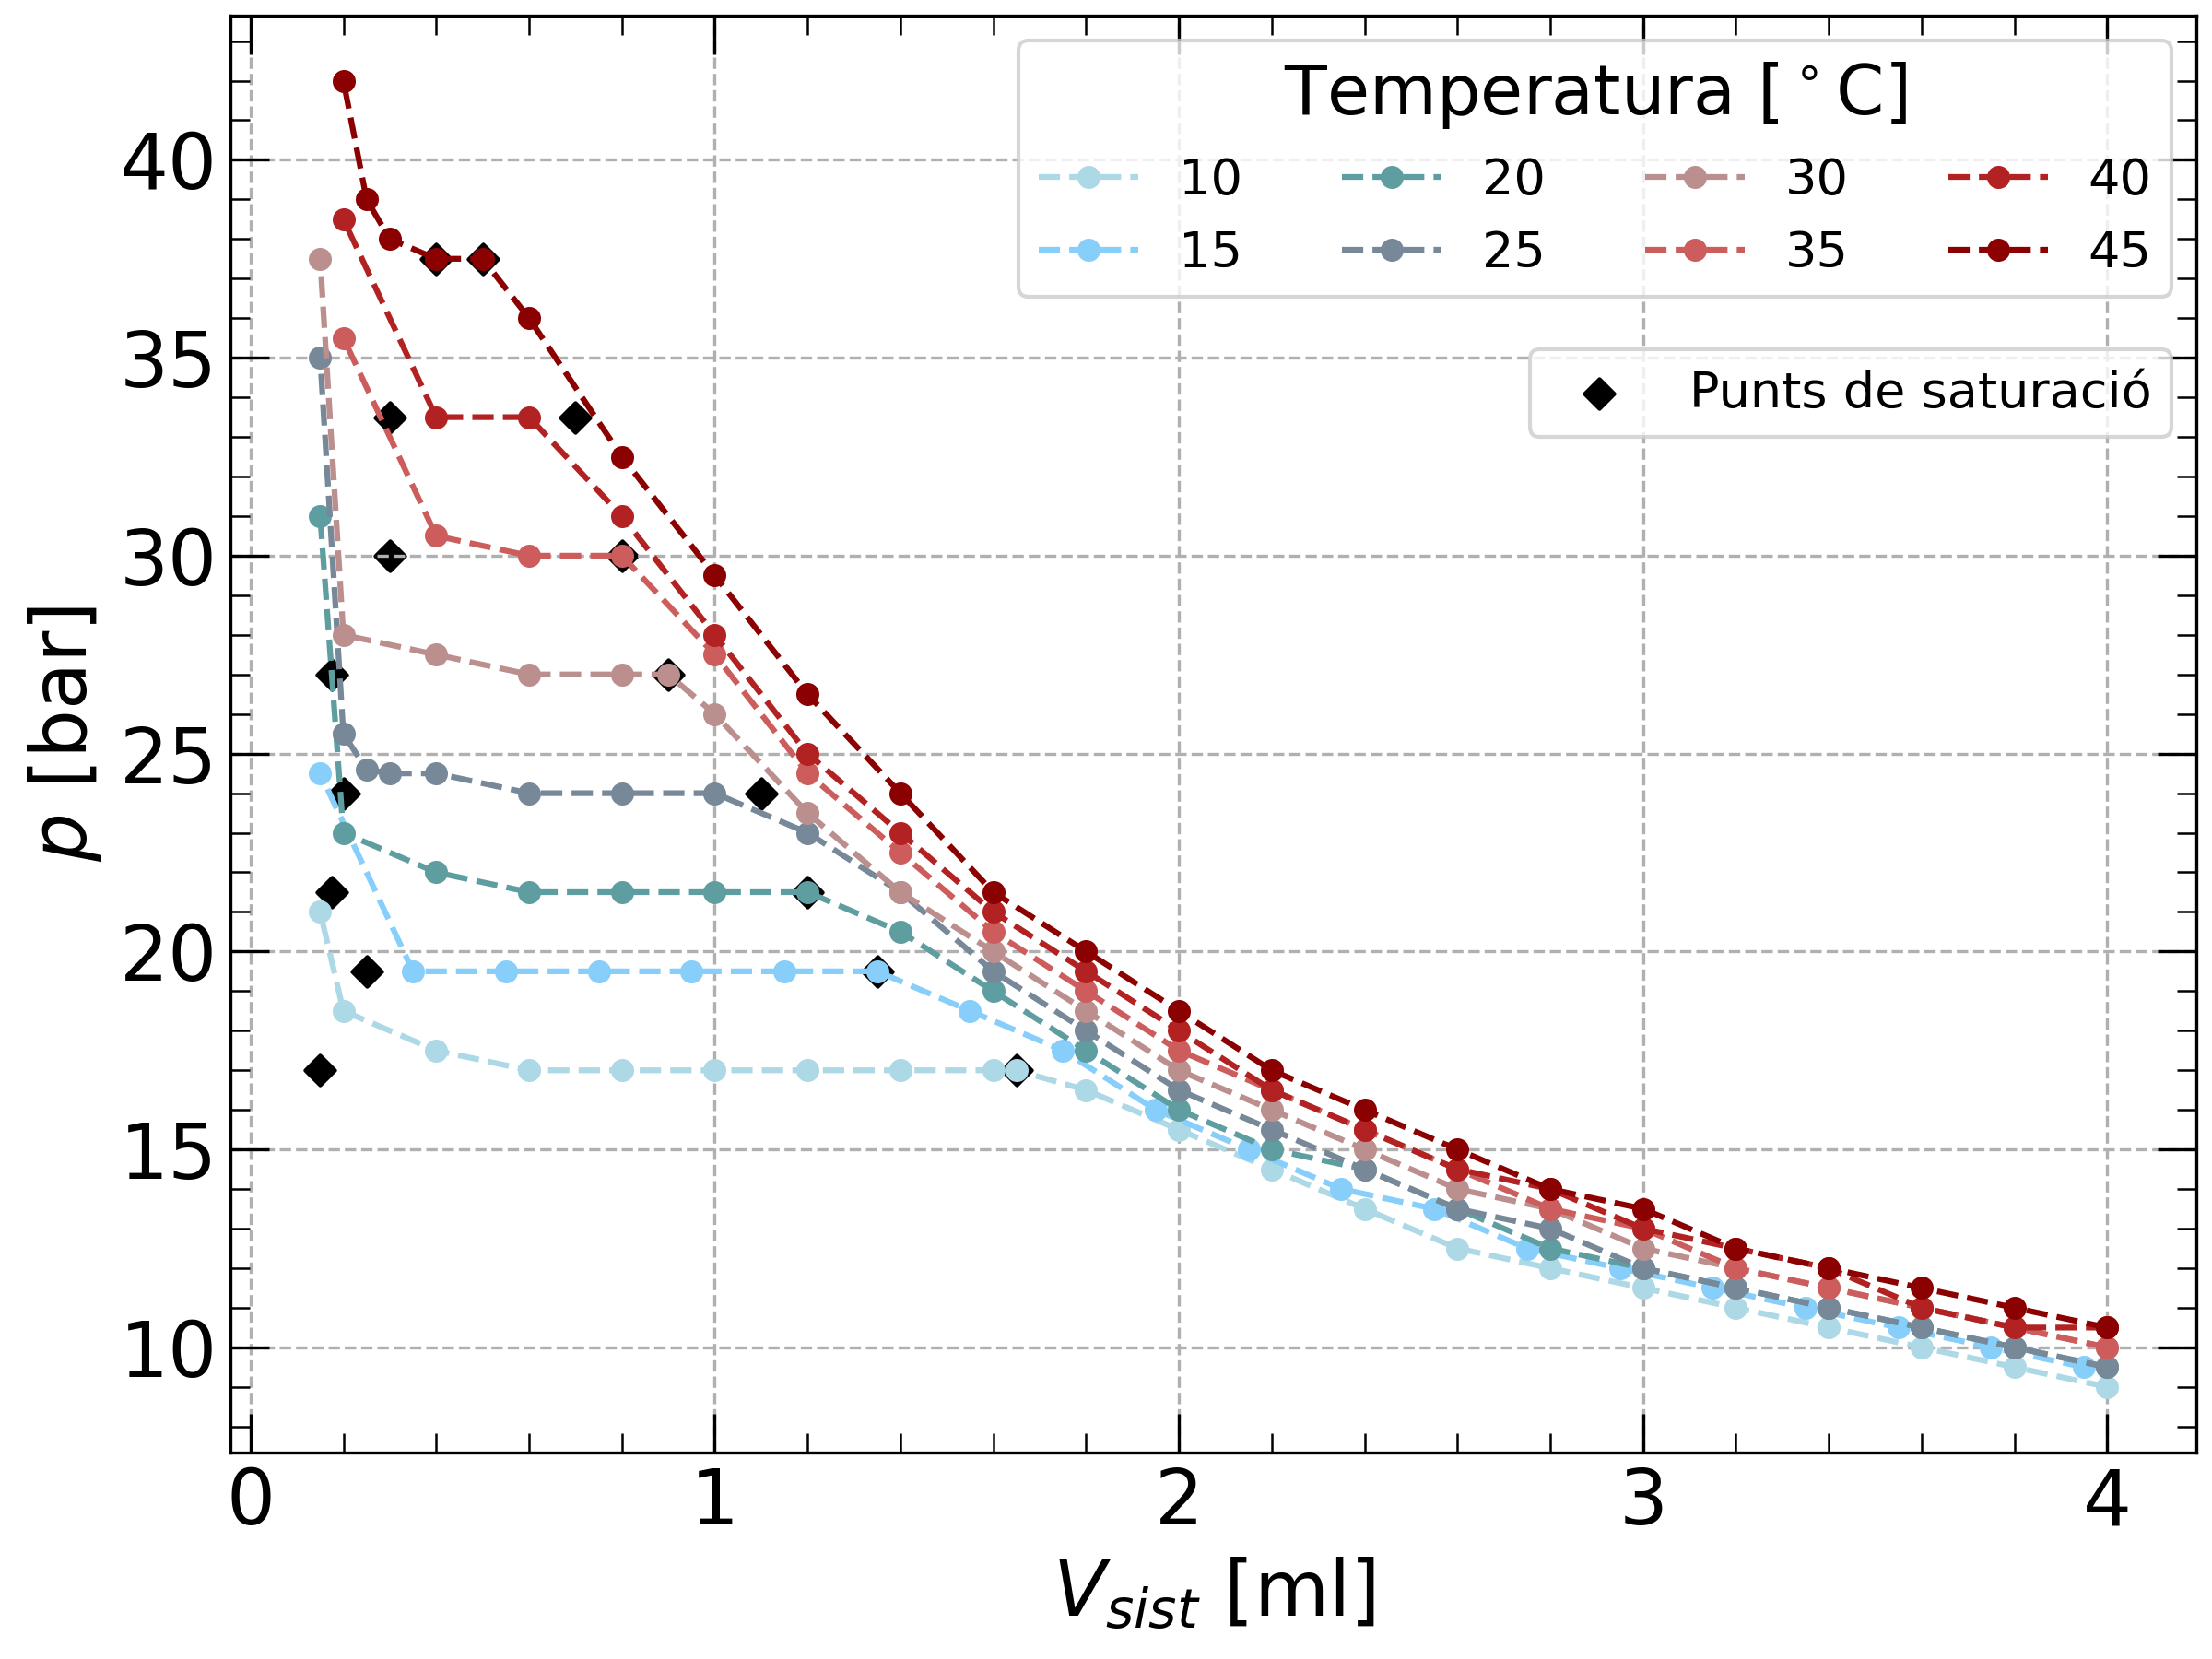
\includegraphics[width=1\linewidth]{../../graphs/practica_IIIb/plots/Clapeyron.png}
  \captionof{figure}{\footnotesize Diagrama de Clapeyron $p$ vs. $V_{sist}$ per a diferents temperatures i punts de la corba de saturació (color negre) a partir de mesures experimentals. Es representen les temperatures amb un degradat de color, des de blau per a la temperatura més baixa fins a vermell per a la més alta. Notem com les isotermes ascendeixen amb la temperatura.}\label{fig:Diagrama_Clapeyron}
\end{Figura}
Amb l'objectiu de trobar el valor de $p$, $V$ i $T$ crítics segons les nostres dades experimentals podem intentar predir el comportament de la corba que marquen els punts de saturació. S'observen els punts de saturació a la Figura \ref{fig:saturacio}, juntament amb un ajust polinòmic de tercer grau. Els coeficients de l'ajust polinòmic queden reflectits a la Taula \ref{tau:coef_poly3}.
\renewcommand{\arraystretch}{1.48}
\begin{Figura}
  \centering
  \captionof{table}{\footnotesize{Coeficients de la regressió polinòmica ($y=\alpha x^3 + \beta x^2 + \gamma x + \delta$) de la corba de saturació.}}
  \resizebox{\textwidth}{!}{
  \begin{tabular}{c|c}
    Coeficient & Valor ajustat\\
    \hline\hline
    $\alpha$ & \((0,51\pm0,12)\cdot10^{-2}\,\text{bar}/\text{ml}^{3} \)\\
    $\beta$ & \((-1,56\pm0,32)\cdot10^{-2}\,\text{bar}/\text{ml}^{2} \)\\
    $\gamma$ & \((1,28\pm0,32)\cdot10^{-2}\,\text{bar}/\text{ml} \)\\
    $\delta$ & \((0,042\pm0,044)\cdot10^{-2}\,\text{bar} \)
  \end{tabular}
  }
  \label{tau:coef_poly3}
\end{Figura}
\renewcommand{\arraystretch}{1}
Observem com el coeficient $r^2$ dona un valor molt baix. Aquest resultat ens indica que les mesures que hem pres no són lo suficientment precises i que la corba de saturació no s'ajusta a un polinomi de tercer grau. Si intentem augmentar o disminuir el grau del polinomi al qual s'ajusta la corba arribem a resultats incoherents, a diferència de com veurem a continuació. La decisió de fer servir un polinomi de tercer grau radica en obtenir simplicitat en les expressions i no realitzar un sobreajust de les dades. No tenim informació suficient per a proposar un candidat que s'ajusti perfectament. Augmentar el grau del polinomi provoca que $r^2$ millori (realitzant-ho per a un polinomi de quart grau, aquest pren un valor de \(r^2 =  0,823\)) i, de fet, la corba ajusta molt millor els punts. Però, fent això perdem informació i significat físic, augmentar el grau ajusta la corba a les oscil·lacions d'error experimental i comporta a un augment molt significatiu de l'error dels coeficients ajustats.\\\\
A partir dels coeficients de l'ajust de tercer grau podem tractar la corba com si fos aquest polinomi. Derivant i igualant a zero obtenim el valor de $V_c$ experimental. Per a realitzar-ho apliquem el mètode de Newton-Raphson, obtenint que
\begin{equation*}
  V_c = (0,6\pm0,2) \, \text{ml}
\end{equation*}
Trobat aquest valor, podem trobar $p_c$ experimental substituint $V_c$ al polinomi, obtenint
\begin{equation*}
  p_c = (36\pm21) \, \text{bar}
\end{equation*}
S'observa com a causa del gran error obtingut a l'ajust de la corba de saturació l'error calculat de la pressió crítica surt molt alt. Tot i això, el valor obtingut és comparable amb les dades tabulades de la literatura, com es veu més endavant.
\begin{Figura}
  \centering
  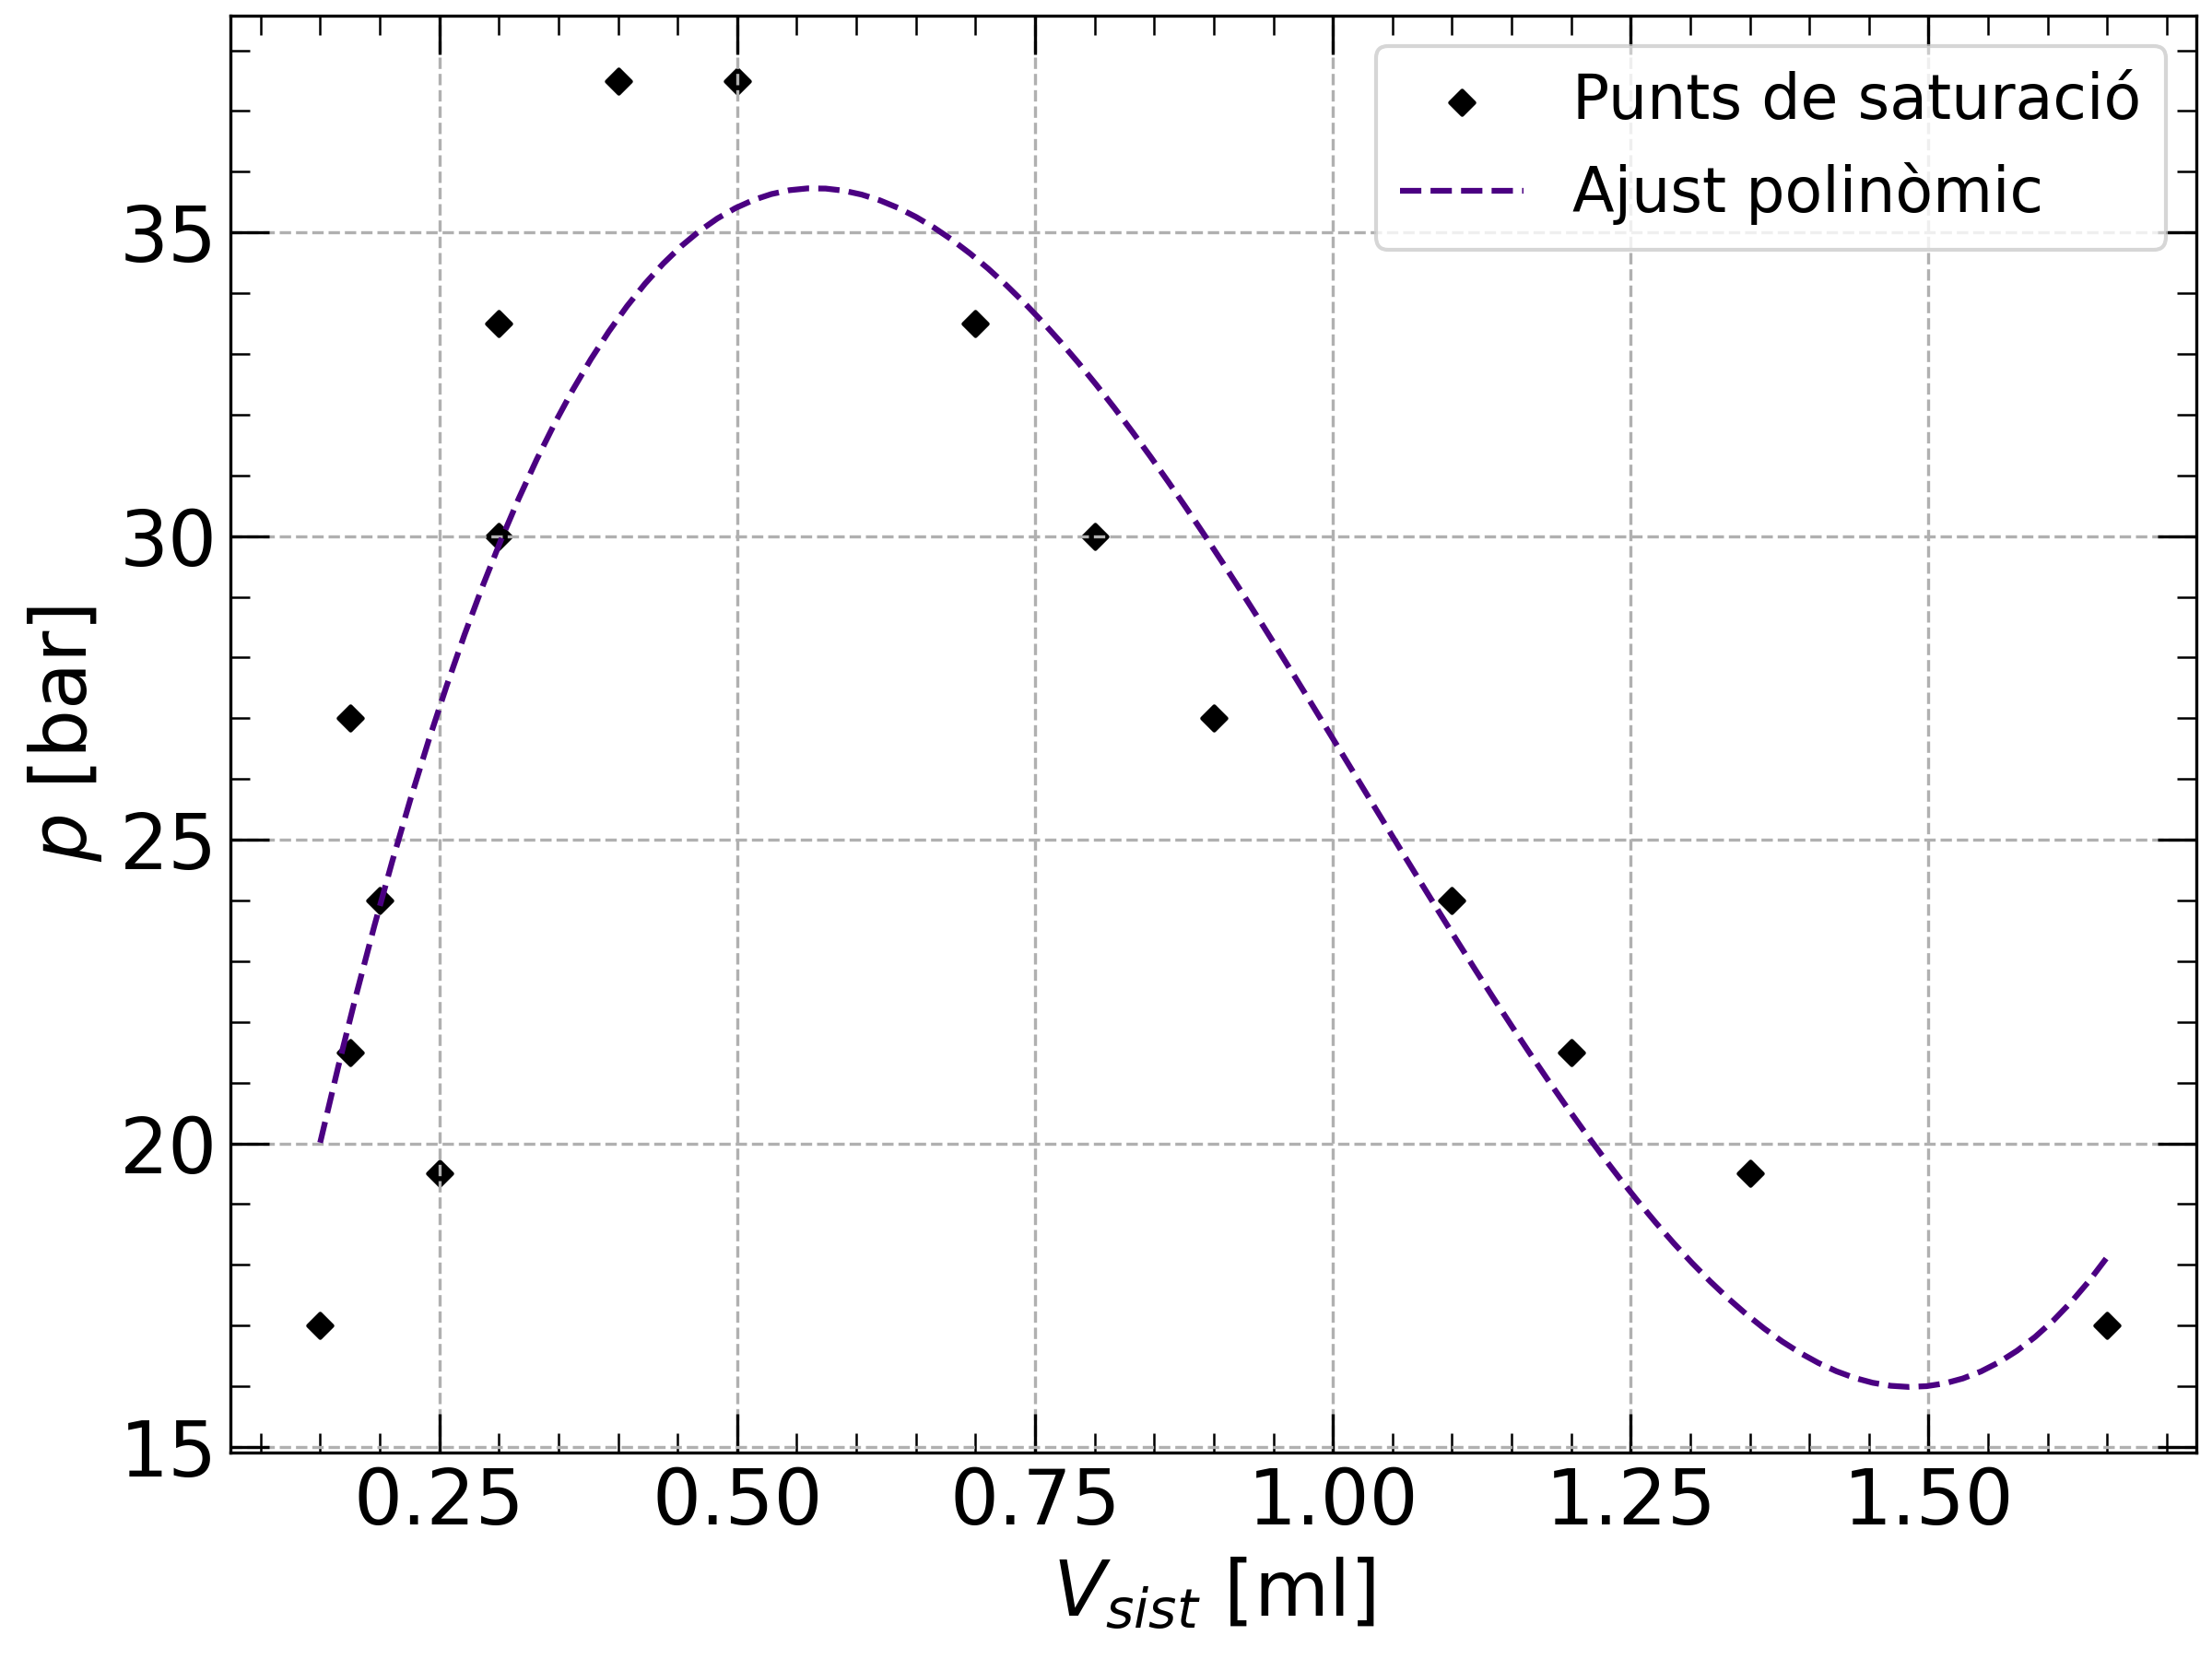
\includegraphics[width=\linewidth]{../../graphs/practica_IIIb/plots/Corba_Saturacio.png}
  \captionof{figure}{\footnotesize{Punts experimentals de la corba de saturació i regressió polinòmica. Regressió amb un coeficient $r^2=0,788$.}}
  \label{fig:saturacio}
\end{Figura}
Per a trobar la temperatura crítica treballarem amb les dades $p$-$T$ experimentals. Tot i que amb excepcions, les dades $p$-$V$ mesurades per a cada temperatura s'han realitzat amb el mateix pas de volum, això es pot observar a la Figura \ref{fig:Diagrama_Clapeyron}. Sabent això podem graficar els punts $p$-$T$ per les pressions de vapor al canvi de fase. Podem observar la relació entre pressió i temperatura a primer ordre on, segons l'Equació \eqref{Clausius}, ha de tenir un comportament lineal. S'observa a la Figura \ref{fig:reg_p_vs_T} com pressió i temperatura tenen un comportament lineal.
\begin{Figura}
  \centering
  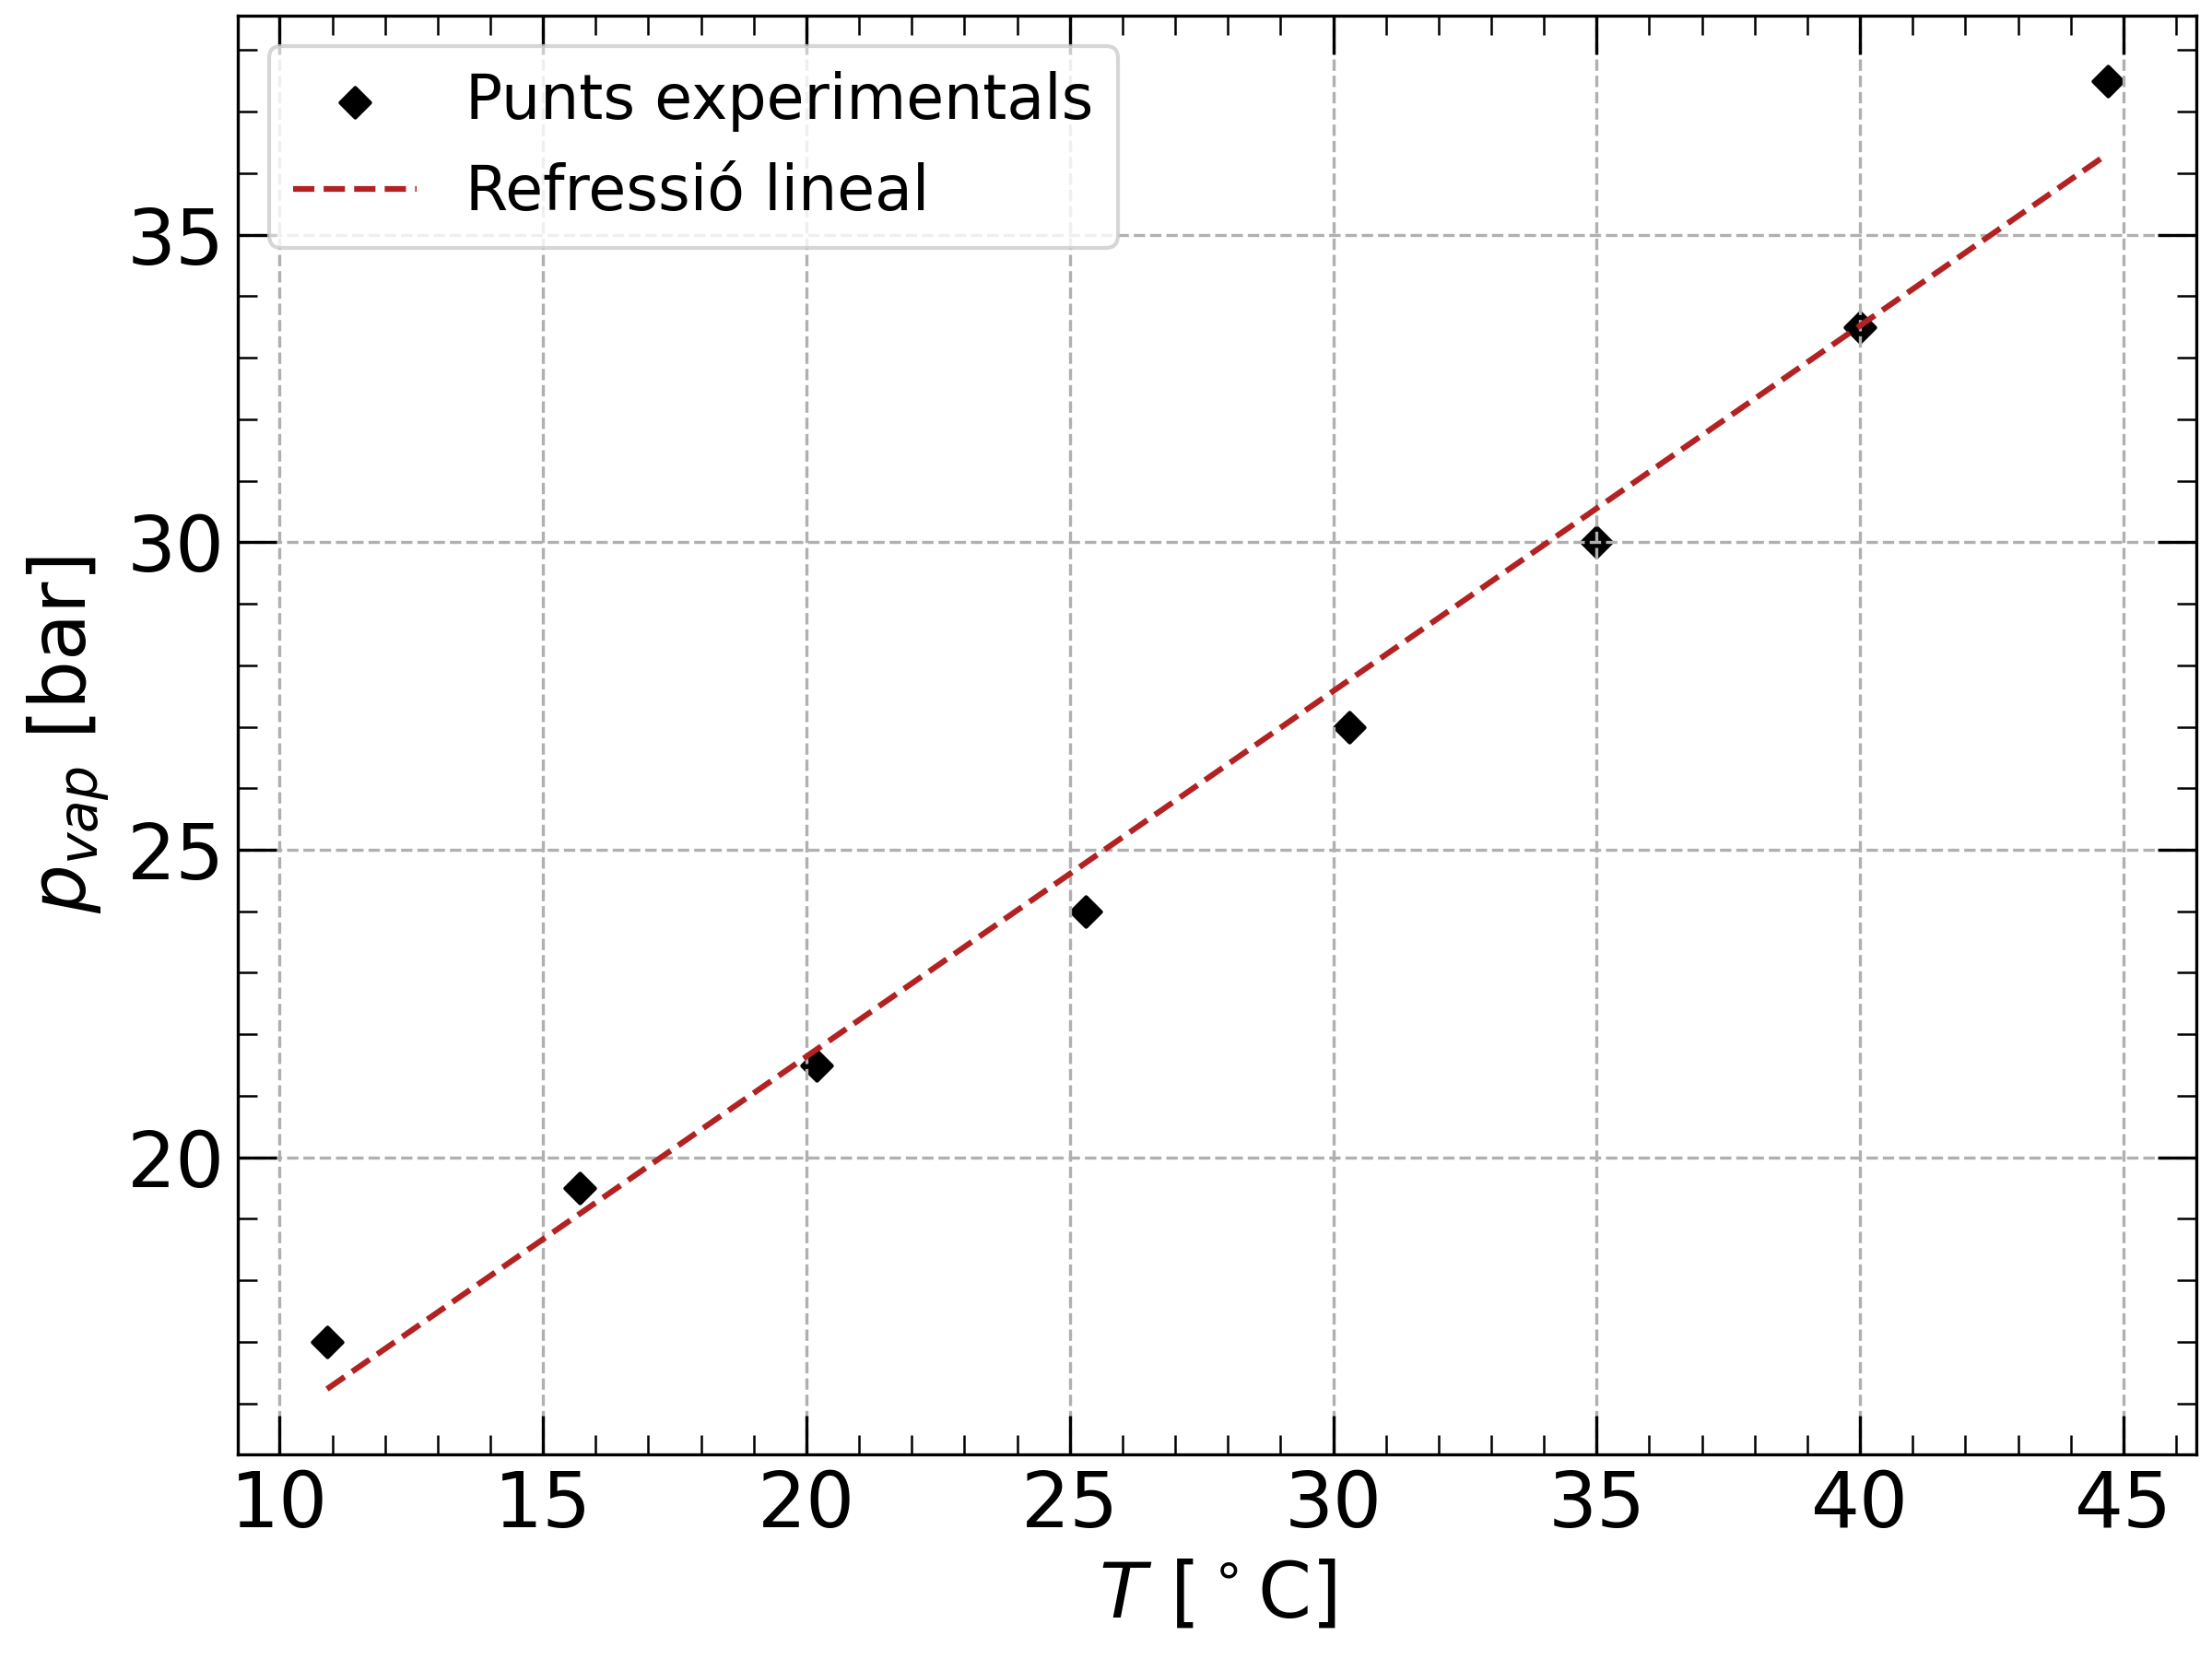
\includegraphics[width=\linewidth]{../../graphs/practica_IIIb/plots/p_vs_T_vap.png}
  \captionof{figure}{\footnotesize{Punts experimentals i regressió lineal ($y = \bar{a}x + \bar{b}$) de $p_{\text{vap}}$ vs $T$. Coeficients de regressió: \(\bar{a} = (0,59\pm0,03) \, \text{bar}/\text{K}  \), \( \bar{b} = (9,8\pm0,8) \, \text{bar} \). Regressió amb un coeficient $r^2=0,989$}}
  \label{fig:reg_p_vs_T}
\end{Figura} 
A partir de descriure pressió i temperatura de forma lineal amb els coeficients obtinguts i del valor que acabem de calcular de $p_c$ obtenim
\begin{equation*}
   T_c = (317\pm35) \, \text{K}
\end{equation*}
on s'observa també un valor d'error molt alt derivat del càlcul de $p_c$. Per a poder comparar amb valors tabulats a la literatura, es plasmen aquests resultats a la Taula \ref{tau:comparacio_Exp}.
\renewcommand{\arraystretch}{1.57}
\begin{Figura}
  \centering
  \captionof{table}{\footnotesize{Taula comparativa de \(p_c\,(\text{bar})\), \(T_c\,(\text{K})\) i \(v_c\,(\text{L}/\text{mol})\) entre les dades tabulades a la literatura i les obtingudes experimentalment.}}
  \resizebox{\textwidth}{!}{
  \begin{tabular}{c|c|c|c}
    \multirow{1}{1.3cm}{} &Exp.\footnotemark & Tab. \cite{NIST} & Tab. \cite{CRC}\\
    \hline\hline
    $p_c$ & $36\pm21$&37,586&37,7\\
    $T_c$ & $317\pm35$& 318,71 &318,723\\
    $v_c$ & $0,32\pm6,26$ & 0,198 & 0,197\\
  \end{tabular}
  }
  \label{tau:comparacio_Exp}
\end{Figura}
\renewcommand{\arraystretch}{1}
\footnotetext{S'observa com el valor experimental de $p_c$, $T_c$ i $v_c$ no s'expressa correctament segons les seves xifres significatives. A causa de l'error acumulat, el valor mesurat hauria d'expressar-se, per exemple com a zero en el cas de $v_c$. Amb motivació de comparar resultats, s'ignora el problema per a aquests valors, ja que encara conté informació d'interès per a la pràctica.}
El valor experimental de $v_c$ s'obté i es discuteix més endavant, a la Secció \ref{trobar_mols}. Observem com, tot i que les mesures experimentals tenen poca precisió (l'error obtingut és molt gran a causa de l'ajust polinòmic de la corba de saturació) són prou exactes com per a assimilar-se a les dades obtingudes de la literatura. Tot i això, aquesta falta de precisió ens indica que no podem treure conclusions més enllà de les comparatives amb la literatura. Per a obtenir uns resultats experimentals realment satisfactoris, s'hauria de seguir un mètode més exhaustiu, amb un pas de volum més petit i aparells de mesura amb més precisió que solucionin els biaixos qualitatius a l'hora de mesurar.\\\\
Des d'una visió quantitativa es podria realitzar més recerca o fer altres experiments que permetin, no només aplicar mètodes numèrics més precisos per a tractar les noves dades obtingudes, sinó també obtenir models que descriguin la dependència amb la temperatura de magnituds que, en aquesta pràctica, presumim de lineals.\\\\
Per tal de poder visualitzar encara millor el comportament de les fases del SF$_6$ al voltant del punt crític obtingut, realitzem un cicle on modifiquem volum, pressió i temperatura de forma que envoltem el punt crític. Es pogué observar com existeixen zones que delimiten en quin estat es troba el fluid, amb unes fronteres ben definides. El SF$_6$ en coordenades del diagrama de Clapeyron per sota de la corba de saturació es troba de forma heterogènia, conviuen vapor i líquid, això ho trobem a, per exemple, a la transició de fase corresponent a la isoterma a \(T=40\,^\circ\text{C}\). Al realitzar una expansió, per a volums superiors que surtin de la corba de saturació i per a temperatures que no superin la temperatura crítica, el SF$_6$ esdevé únicament vapor. Si en aquest punt del diagrama pujem la temperatura isocòricament, superant la temperatura crítica, observem com el gas adopta una forma que no ens permet distingir si és gas o líquid, ens trobem davant d'un fluid super crític. Realitzem una compressió per sota dels \(0,4 \, \text{ml}\), de forma que assegurem que hem passat la corba de saturació per sobre del punt crític. El comportament de la pressió ara és diferent, no s'observa cap transició i la pressió varia de forma contínua. En traspassar la isoterma crítica observem com passem d'observar un fluid supercrític a simplement un líquid. Per a finalitzar, baixem la temperatura novament als \(40 \, ^\circ\text{C}\) i augmentem el volum fins a tornar al punt de partida. S'observa una caiguda brusca de la pressió i com, al entrar novament sota la corba de saturació, apareix de nou un estat heterogeni de SF$_6$.\\\\
Per tant, hem pogut identificar experimentalment les fronteres que delimiten les fases del SF$_6$ al voltant del punt crític. La fase heterogènia líquid + vapor la delimita la corba de saturació, la trobem en aquelles coordenades per sota de la corba. La fase gasosa la trobem delimitada entre la part dreta (volums alts) superior de la corba de saturació i la isoterma crítica. La fase de fluid supercrític la trobem delimitada per la isoterma crítica, trobant-la a les coordenades per sobre d'aquesta. I, finalment, la fase líquida la trobem a les coordenades per sobre de la part esquerra (volums petits) superior de la corba de saturació i per sota de la isoterma crítica.
\subsection{Diagrama d'Amagat}
Es pot observar a l'Equació \eqref{gas_ideal} com en un gas ideal la funció $pV = f(p)$ és un valor constant (només depèn de $T$), en un diagrama d'Amagat $pV$ vs $p$ s'haurien de veure rectes horitzontals, una per a cada temperatura, les quals augmentarien el valor de l'ordenada a mesura que augmenta la temperatura. A partir de les nostres dades experimentals construïm el diagrama d'Amagat que s'observa a la Figura \ref{fig:amagat}.
\begin{Figura}
  \centering
  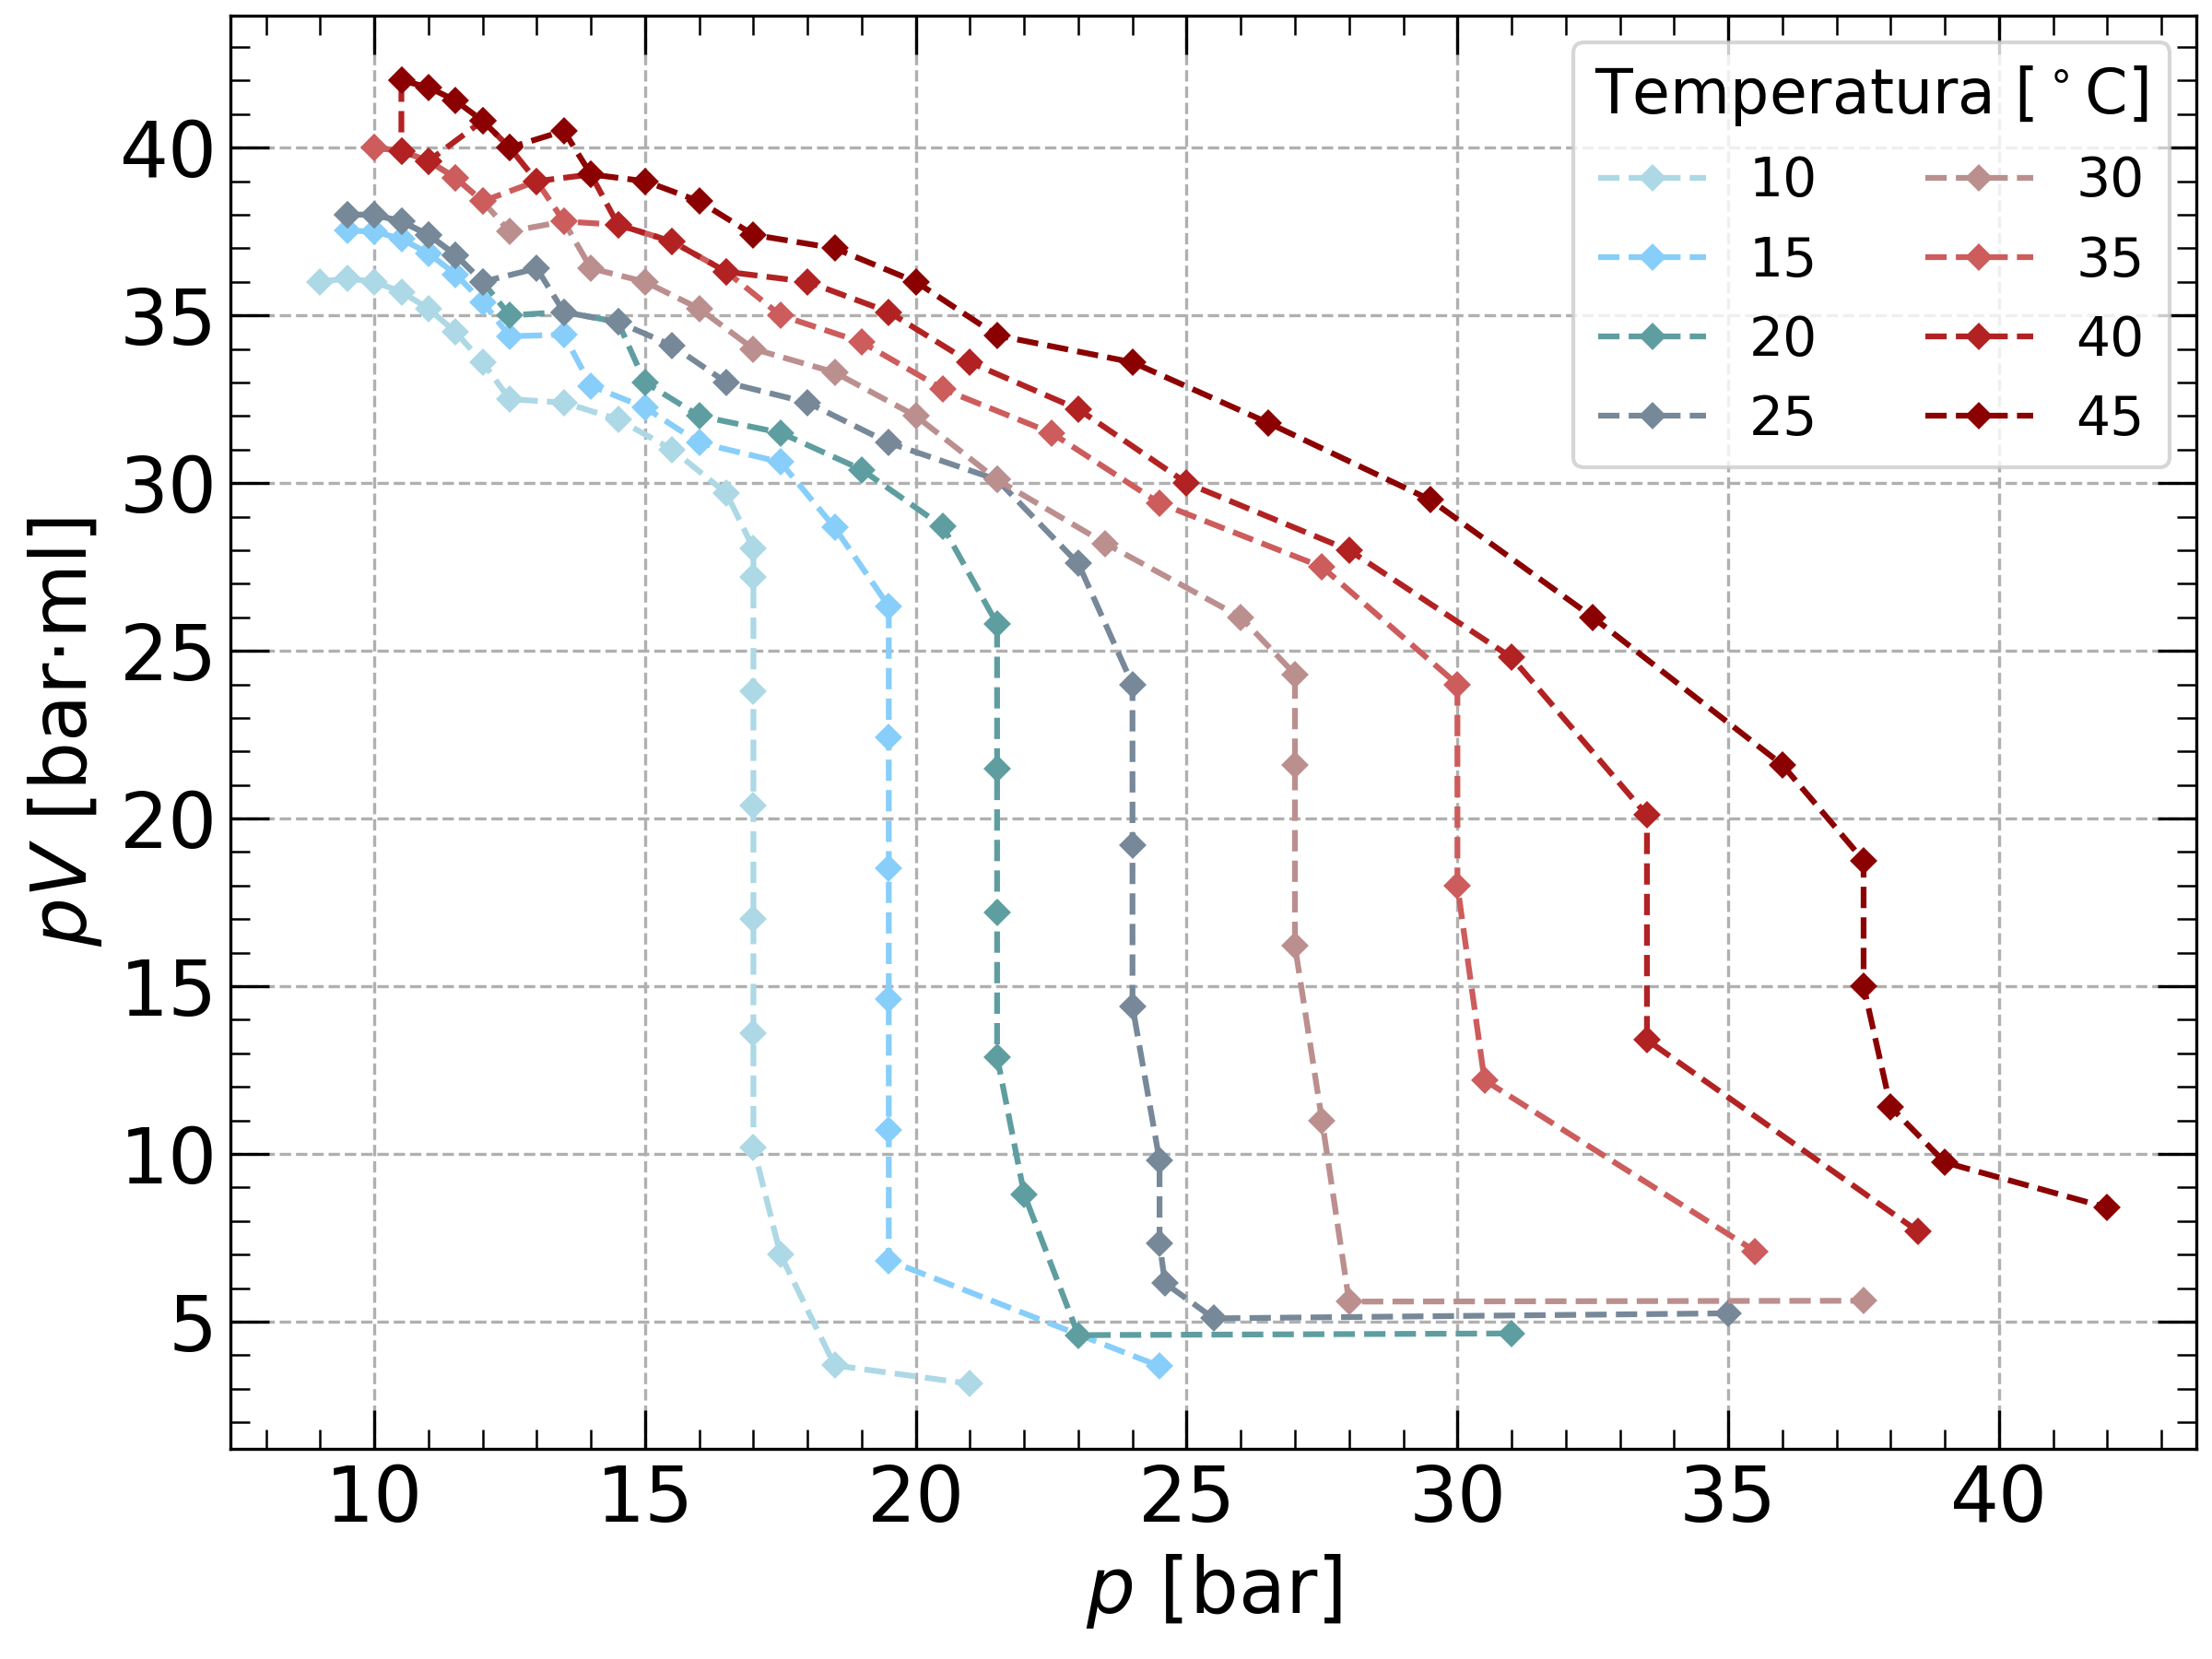
\includegraphics[width=\linewidth]{../../graphs/practica_IIIb/plots/Amagat.png}
  \captionof{figure}{\footnotesize{Diagrama d'Amagat $pV$ vs $p$ per a diferents temperatures a partir de les dades experimentals. Es representen les temperatures amb el mateix degradat de color que la Figura \ref{fig:Diagrama_Clapeyron}. S'observa com la corba decau seguint un patró similar per a cada temperatura. També es veu com, segons la temperatura, a altes pressions el comportament de la corba d'Amagat sembla ser el d'una recta amb valor constant.}}
  \label{fig:amagat}
\end{Figura}
Observem que el comportament de les nostres dades experimentals no segueixen la predicció d'un gas ideal. De fet, la corba que fan les dades a cada temperatura adopta una forma complicada, però es pot observar com hi ha un patró que es repeteix per a cada temperatura. Podem notar com aquesta dependència de l'ordenada inicial amb la temperatura sí que apareix, a mesura que augmenta la temperatura s'observa com la corba es desplaça cap a dalt i cap a la dreta de la gràfica. A més, cada corba arriba fins a un punt $p$ on $pV$ decau bruscament, de forma pràcticament vertical. Aquests punts de pressió coincideixen amb el valor de pressió de vapor corresponents al canvi d'estat vapor-líquid del SF$_6$.
\subsection{Diagrama $pV$ vs $1/V$. Obtenció del nombre de mols}\label{trobar_mols}
Com hem vist a l'Equació \eqref{virial} es pot treure informació d'un gas real a partir del seu desenvolupament del virial. Per a obtenir el nombre de mols del nostre sistema farem servir el desenvolupament del virial aproximat com s'ha vist a l'Equació \eqref{virial_tallat}. D'aquesta manera, per a un tram lineal a prop del zero d'un diagrama $pV$ vs $1/V$ (és a dir, per a volums grans) podem realitzar una regressió i obtenir el nombre de mols a partir de l'ordenada d'origen. A la Figura \ref{fig:pV_vs_1_V} es mostra aquest diagrama fet a partir de les nostres dades experimentals. Es pot observar com existeix aquest tram lineal a $V^{-1}$ petites.\\\\
També s'observa que a mesura que disminueix el volum el comportament de les corbes tendeix a aplanar-se. Això es pot explicar veient que l'Equació \eqref{virial} depèn de termes més enllà de primer ordre. Aquest aplanament correspon, en el diagrama de Clapeyron, a la zona on el SF$_6$ es troba en fase líquida.\\\\
Per a obtenir les dades necessàries i aproximar les rectes que busquem fem diverses iteracions. Per a cada temperatura es genera una llista de dades $pV$ i $V^{-1}$ amb $k$ entrades de la quantitat total de valors que hem mesurat. Començant per $k = 3$ (per a poder dibuixar una recta i assegurar que a la primera no obtenim un valor de $r^2=1$ a causa de només tenir dos valors experimentals) calculem el valor $r^2$ per a cada $k$-llista. De les $r^2$ obtingudes prenem com a bon ajust aquella que és màxima, i s'acaba fent la regressió d'aquell nombre de punts que maximitzen $r^2$. \\\\
Les dades obtingudes d'aquest procediment es veuen reflectides a la Taula \ref{tau:dades_iteracio_reg}, i a la Figura \ref{fig:dades_itercio_reg} s'observa el comportament lineal d'aquesta regió del diagrama $pV$ vs $V^{-1}$.
\begin{Figura}
  \centering
  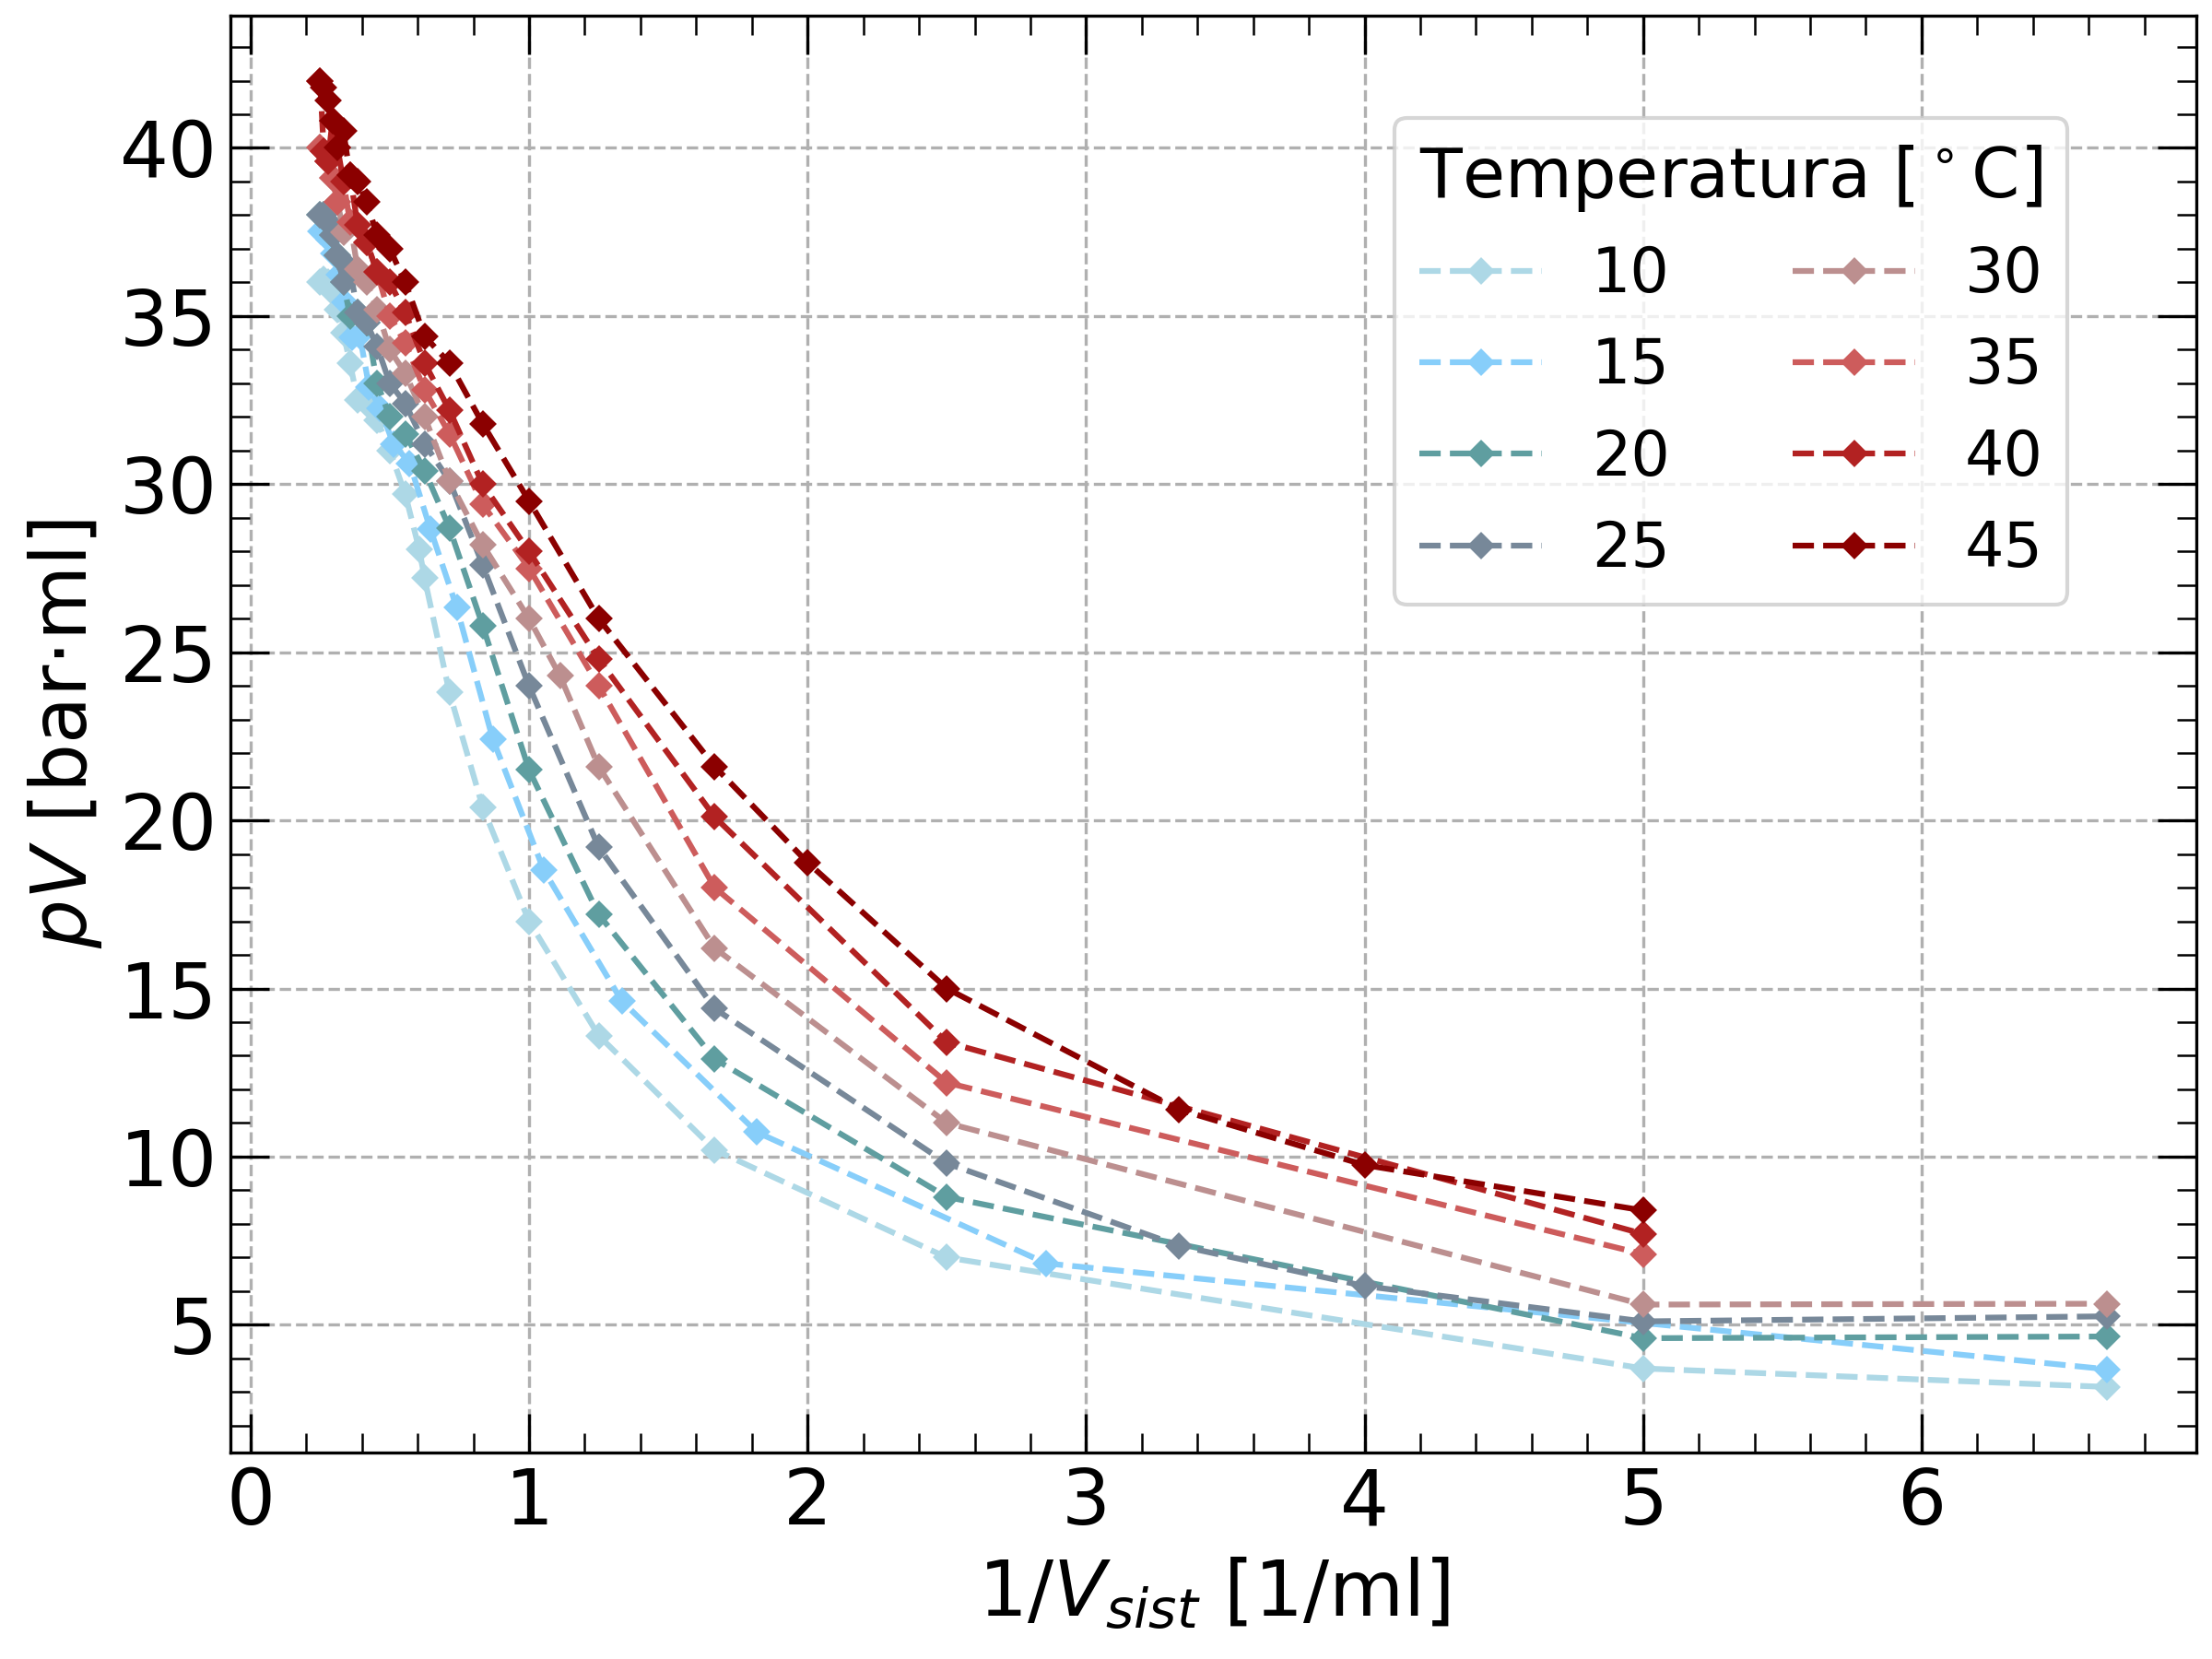
\includegraphics[width=\linewidth]{../../graphs/practica_IIIb/plots/pV_vs_V(-1).png}
  \captionof{figure}{\footnotesize{Diagrama $pV$ vs $V^{-1}$ per a diferents temperatures a partir de les dades experimentals. Es representen les temperatures amb el mateix degradat de color a la Figura \ref{fig:Diagrama_Clapeyron}. S'observa com a volums alts el comportament és aparentment lineal.}}
  \label{fig:pV_vs_1_V}
\end{Figura}
\end{multicols}
\vspace{1.6cm}
\begin{table}[h]
  \centering
  \caption{\footnotesize{Valors òptims de regressió lineal ($y=\bar{a}x+\bar{b}$) de la part lineal del diagrama  $pV$ vs $V^{-1}$ i nombre de mols obtingut per a cada temperatura.}}
  \renewcommand{\arraystretch}{1.85}
  \begin{tabular}{c|c|c|c|c}
     \multirow{1}{2cm}{\centering $T$ [$^\circ$C]} & \multirow{1}{2.8cm}{\centering $\bar{a}$ [bar$\cdot$ml$^{2}$]} & \multirow{1}{2.8cm}{\centering $\bar{b}$ [bar$\cdot$ml]} & \multirow{1}{2cm}{\centering $r^2$} & \multirow{1}{2.8cm}{\centering $n$ ($\cdot 10^{-3}$) [mol]} \\
     \hline\hline
     10 & $-23,3\pm0,8$ & $42,2\pm0,4$ & 0,990 & $1,598\pm0,013$ \\
     15 & $-23,4\pm0,9$ & $43,5\pm0,4$ & 0,996 & $1,842\pm0,016$ \\
     20 & $-21,0\pm0,9$ & $43,2\pm0,4$ & 0,995 & $1,799\pm0,016$ \\
     25 & $-18,0\pm0,6$ & $42,5\pm0,3$ & 0,996 & $1,741\pm0,011$ \\
     30 & $-20,7\pm0,6$ & $44,9\pm0,3$ & 0,990 & $1,810\pm0,011$ \\
     35 & $-19,1\pm0,9$ & $44,9\pm0,3$ & 0,994 & $1,778\pm0,013$ \\
     40 &  $-19,4\pm1,2$  & $45,7\pm0,5$ & 0,979 & $1,78\pm0,02$ \\
     45 & $-18,6\pm0,7$ & $46,3\pm0,3$ & 0,988 & $1,778\pm0,012$ 
           
  \end{tabular}
  \renewcommand{\arraystretch}{1}
  \label{tau:dades_iteracio_reg}
\end{table}
\vfill
\newpage
\begin{multicols}{2}
Es pot observar tant als valors que pren $r^2$ a la darrera taula com al comportament dels punts experimentals a la Figura \ref{fig:dades_itercio_reg} com no totes les temperatures arriben a descriure idealment un comportament lineal. D'igual manera, els valors obtinguts són una bona aproximació a primer ordre.
\begin{Figura}
  \centering
  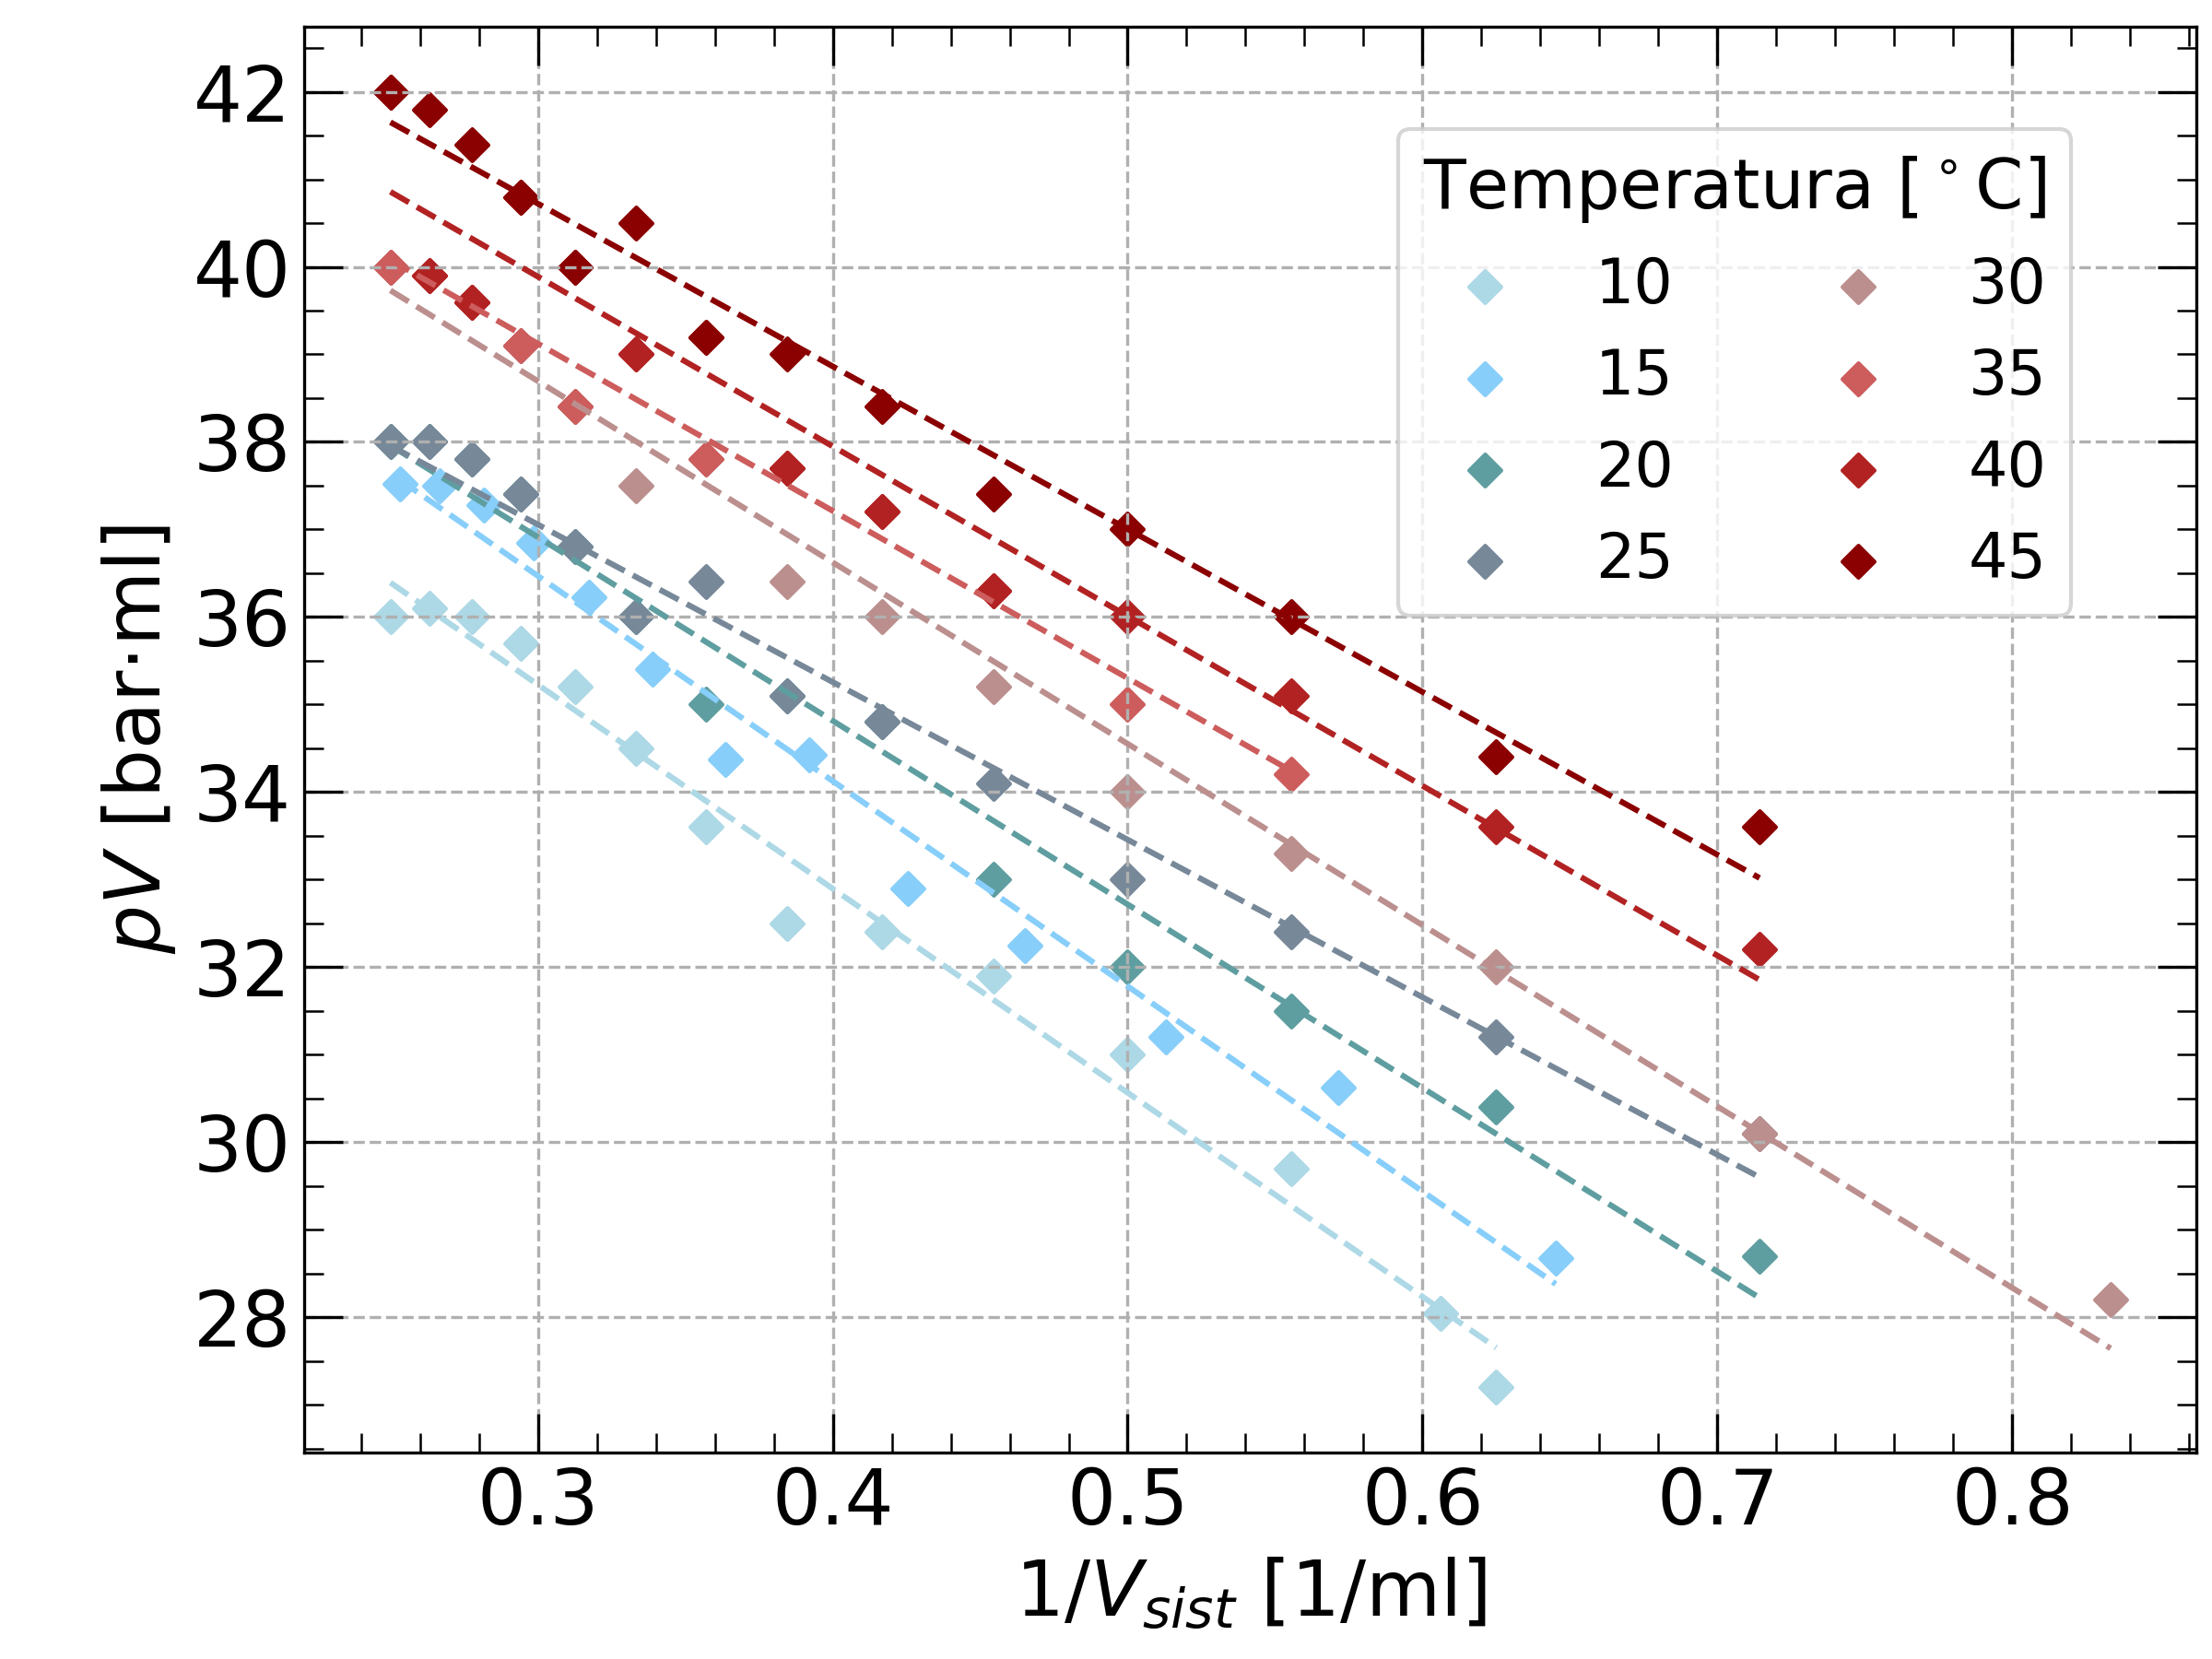
\includegraphics[width=\linewidth]{../../graphs/practica_IIIb/plots/regs_virial.png}
  \captionof{figure}{\footnotesize{Representació i regressions de la part lineal de $pV$ vs $V^{-1}$ per a cada temperatura. S'observa com les dades no segueixen estrictament un comportament lineal. Els coeficients de regressió es troben a la Taula \ref{tau:dades_iteracio_reg}.}}
  \label{fig:dades_itercio_reg}
\end{Figura}
Seguint l'Equació \eqref{virial_tallat} es calcula el nombre de mols a partir de les dades de regressió de cada temperatura, concretament a partir del valor de $\bar{b}$ per a cada temperatura. Aquests valors també s'observen a la Taula \ref{tau:dades_iteracio_reg}. Com a valor del nombre de mols del nostre sistema ens quedarem amb la mitjana d'aquests valors, per tant
\begin{equation*}
  n = (1,77\pm0,02)\cdot10^{-3} \, \text{mol}
\end{equation*}
Sabent això podem comparar el volum crític molar experimental (prenent com a volum crític el que hem obtingut experimentalment) amb el tabulat a la literatura observant novament la Taula \ref{tau:comparacio_Exp}. És molt notable que l'error experimental obtingut és molt alt i no deixa treure conclusions fermes dels nostres resultats. Tot i això, de forma comparativa veiem que el valor obtingut és de l'ordre dels valors tabulats a la literatura. Per a comprovar la validesa del valor obtingut de mols del nostre sistema, hauríem de, o bé realitzar millors mesures de pressió i volum de les que hem realitzat en aquesta pràctica, o bé dur a terme un altre experiment que ens permeti treballar, per exemple, amb la densitat del SF$_6$ en estat líquid.
\subsection{Model de Van der Waals}
Com hem vist, l'equació de Van der Waals per a un gas real depèn de dos paràmetres $a$ i $b$ que varien segons les característiques de la substància que estem estudiant. Fent servir les dades tabulades que es van presentar a la Taula \ref{tau:comparacio_Exp} (farem servir la primera columna de dades tabulades \cite{NIST}) i les expressions que s'observen a \eqref{coef_VdW} trobem que, en el cas del SF$_6$
\begin{equation*}
  a \simeq 587,29\cdot(10^{4})\, \text{bar}\,\text{ml}^2/\text{mol}^2
\end{equation*}
\begin{equation*}
  b \simeq 65,67\, \text{ml}/\text{mol}
\end{equation*}
Amb aquestes dades podem representar el comportament del SF$_6$ suposant que es comporta com un gas de Van der Waals. Observem aquest comportament a la Figura \ref{fig:SF6_VdW}.
\begin{Figura}
  \centering
  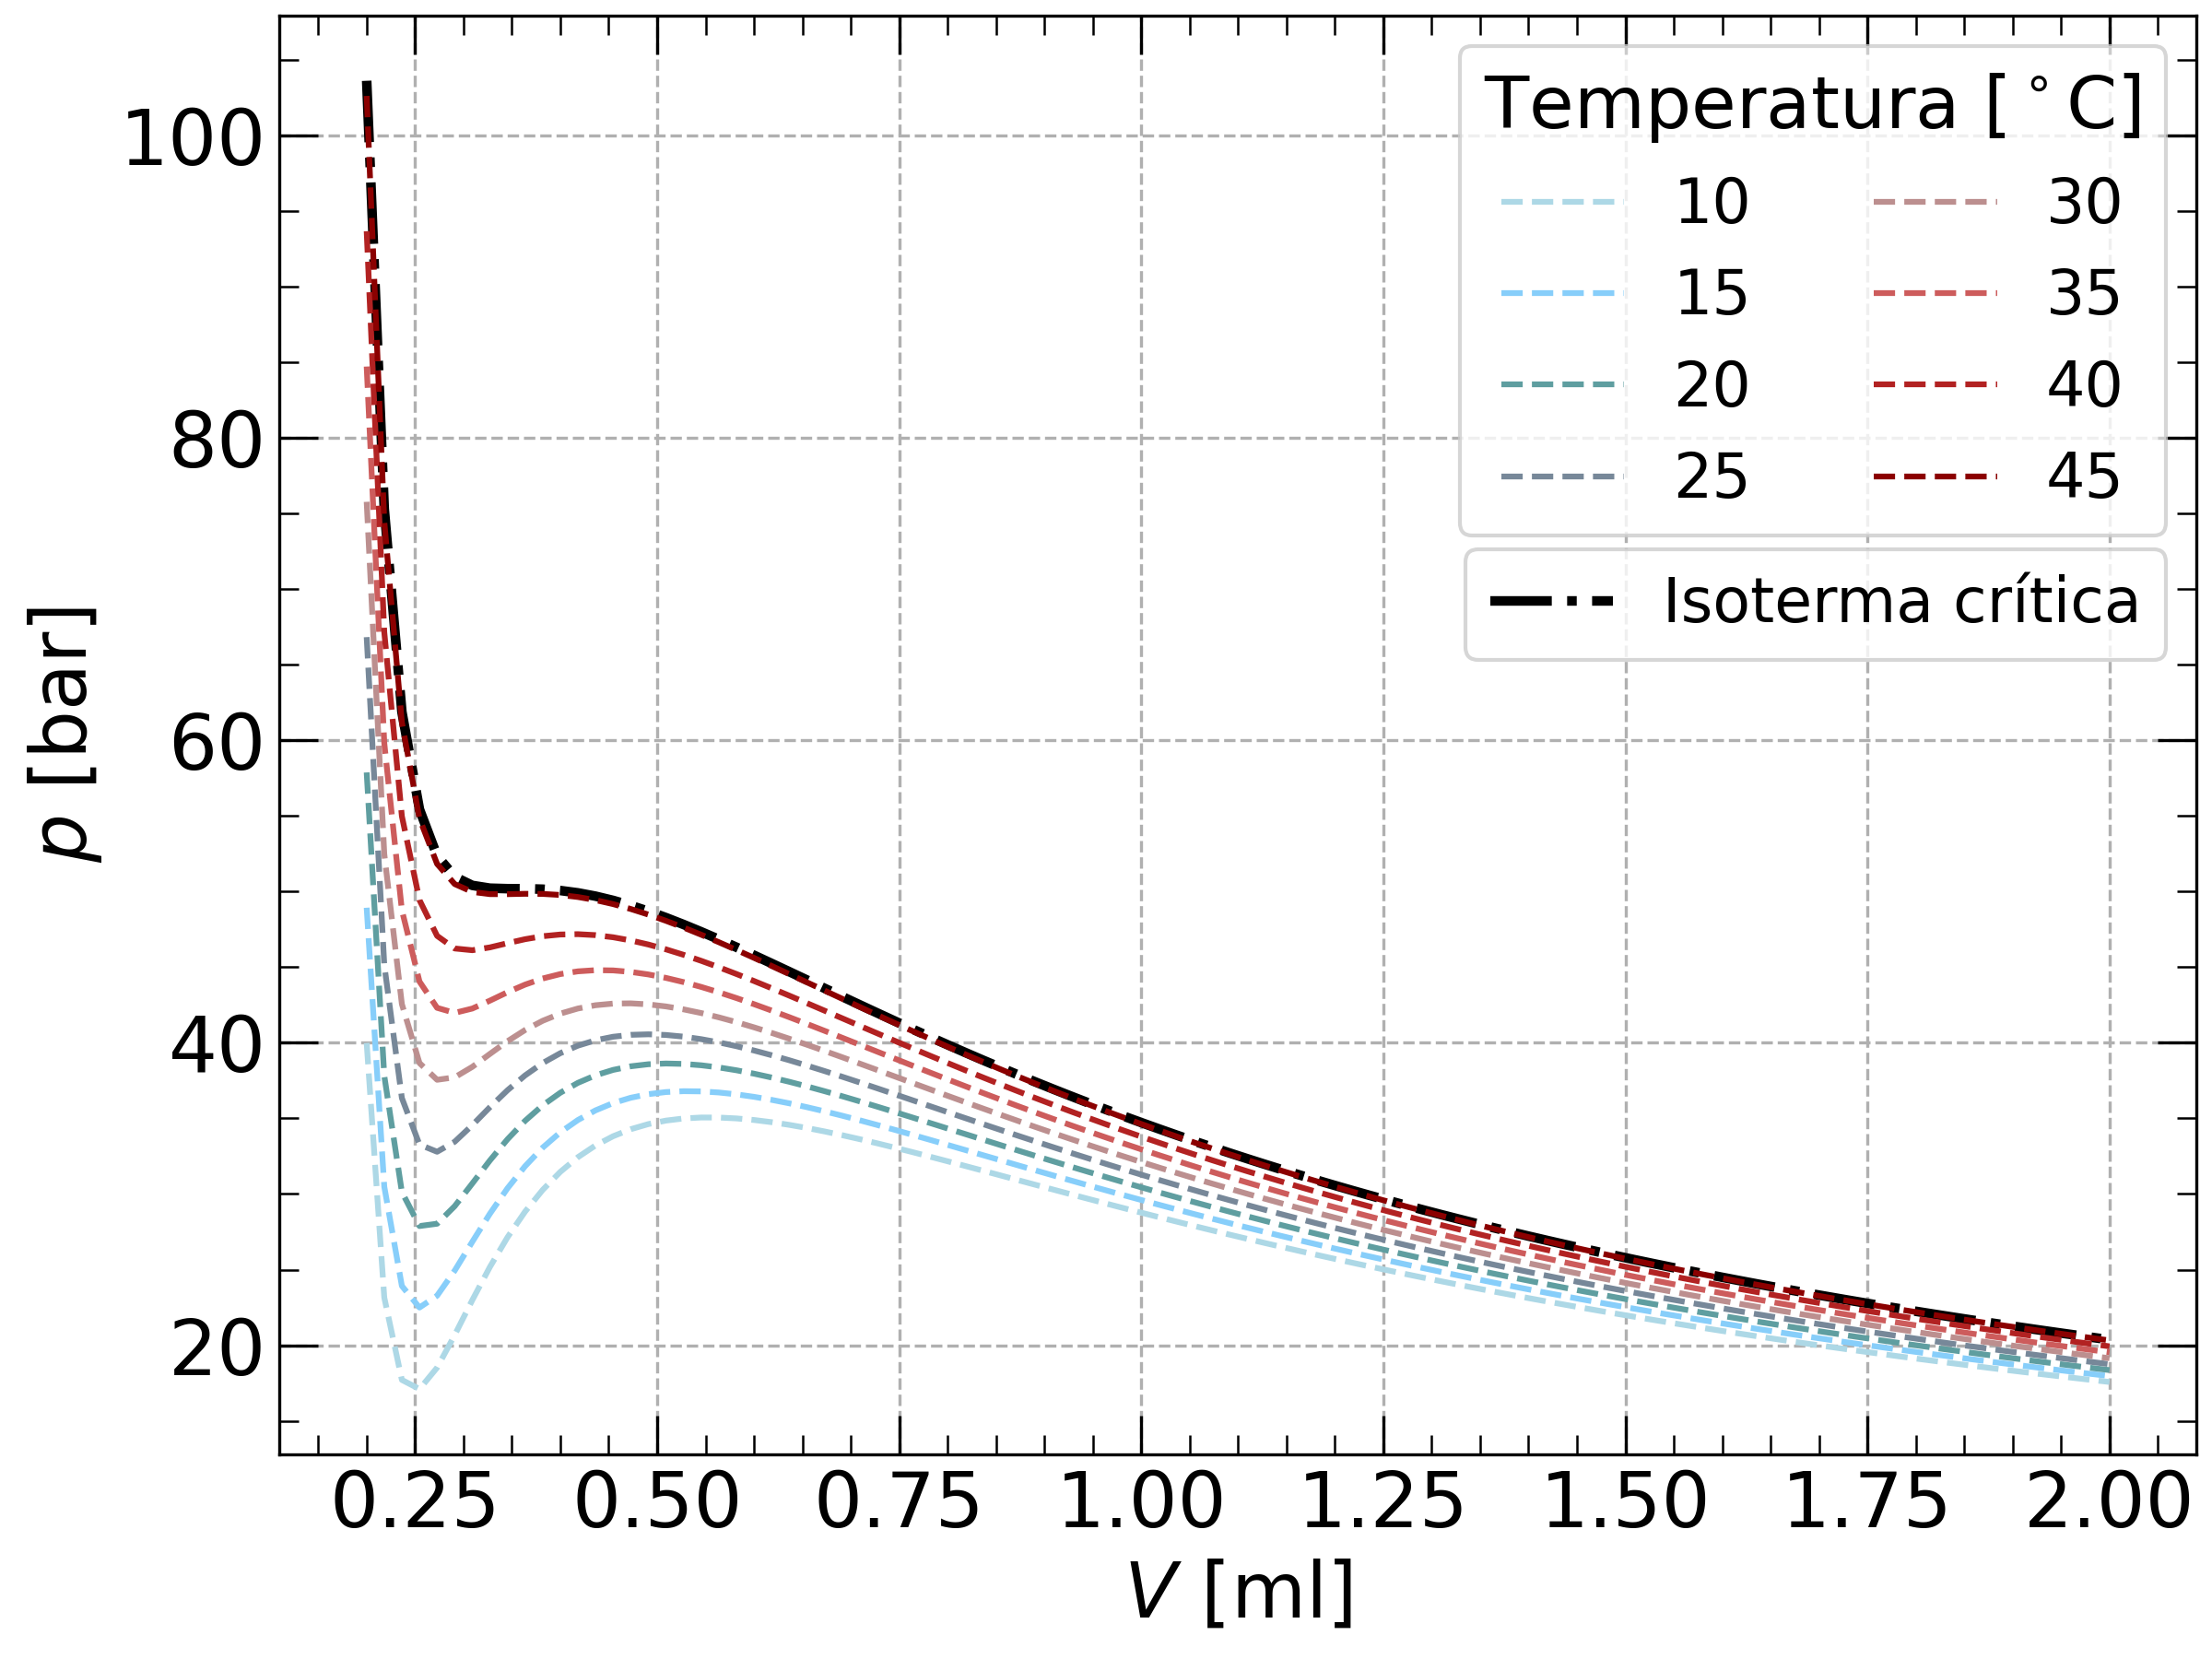
\includegraphics[width=\linewidth]{../../graphs/practica_IIIb/plots/Van_der_Waals.png}
  \captionof{figure}{\footnotesize{Corbes de Van der Waals fetes a partir de les dades tabulades del punt crític del SF$_6$ \cite{NIST}. Per a visualitzar correctament el seu comportament a volums petits, es trunquen les dades fins a arribar a \(2\,\text{ml}\).}}
  \label{fig:SF6_VdW}
\end{Figura}
Observem com aquestes corbes de Van der Waals no prediuen el comportament isobàric durant la transició de fase vapor-líquid del SF$_6$. De fet, com s'ha comentat prèviament, en aquestes corbes hi ha zones on no es compleix l'Equació \eqref{cond_estabilitat}. Aquestes zones corresponen a on el pendent esdevé positiu. A més, també s'observa que la isoterma crítica pren un valor de temperatura més alt del que hauria de ser.\\\\
Amb l'objectiu de poder comparar les corbes obtingudes del gas de Van der Waals amb les nostres dades experimentals i no provocar confusió, a la Figura \ref{fig:comparacio_VdW} s'observen només dues isotermes, una a \(T= 25 \, ^\circ\text{C}\) i altra a \(T= 45 \, ^\circ\text{C}\) (es poden veure la resta d'isotermes a l'Annex).
\begin{Figura}
  \centering
  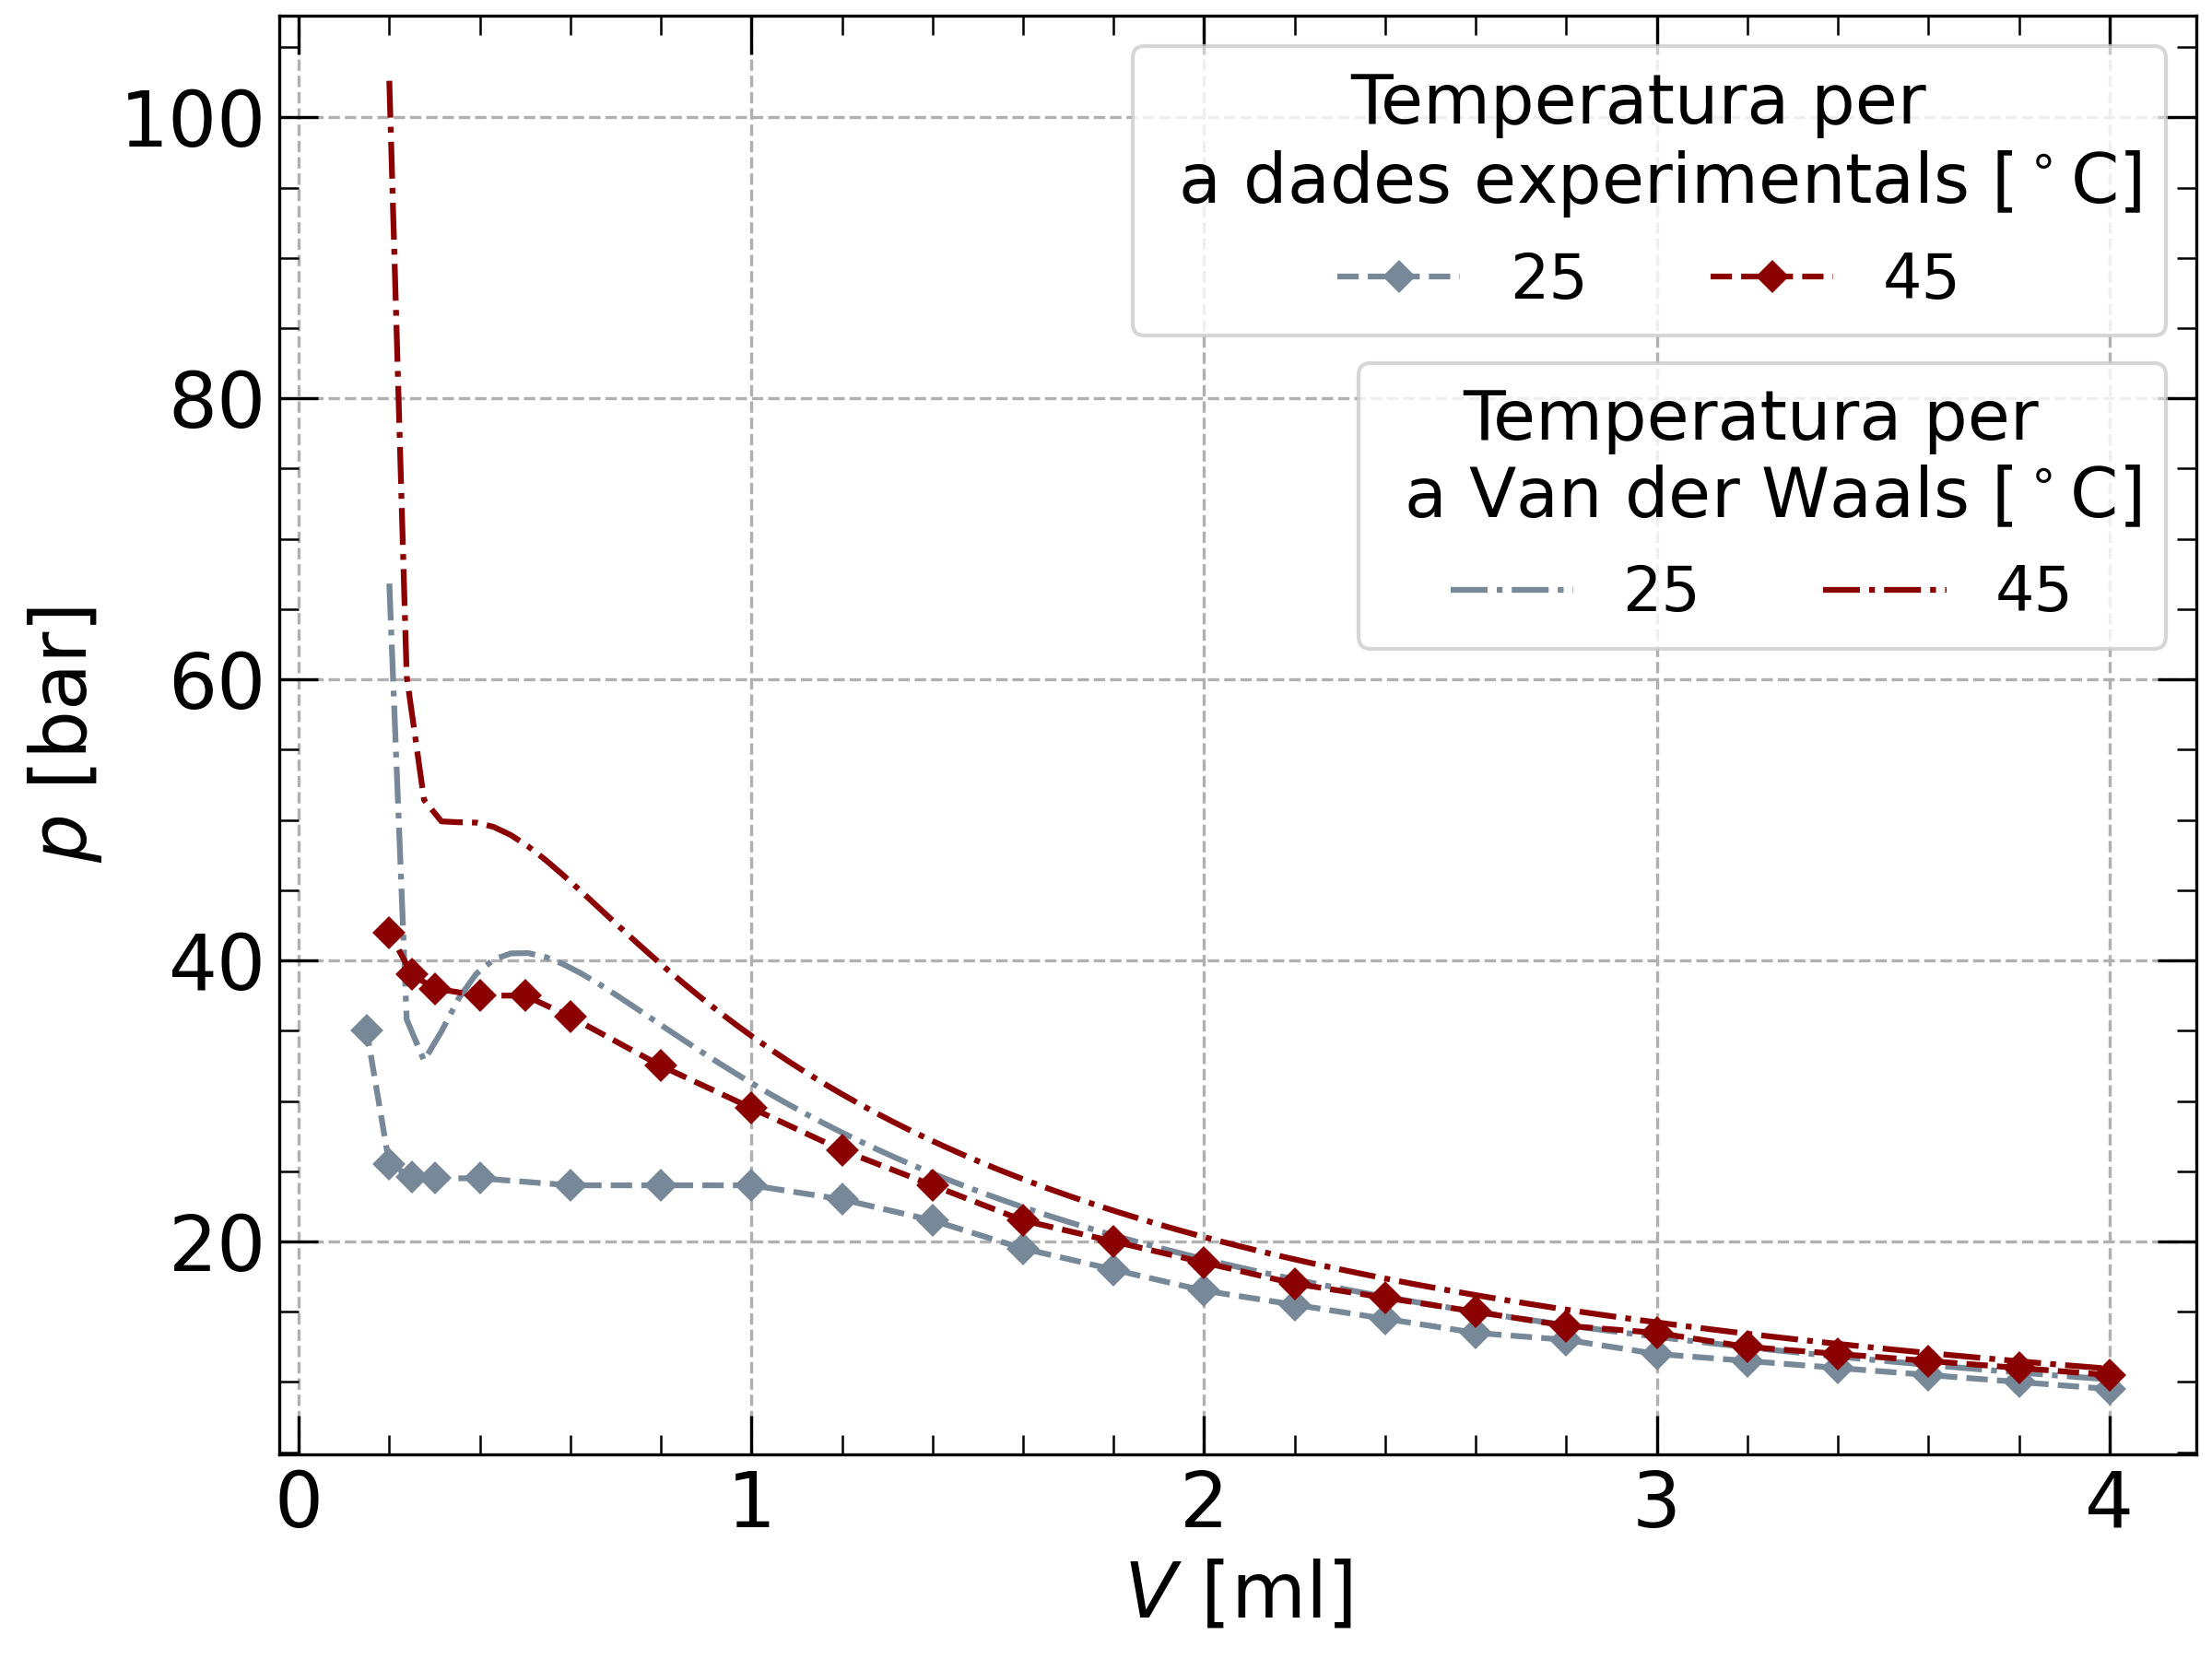
\includegraphics[width=\linewidth]{../../graphs/practica_IIIb/plots/Van_der_Waals_comparativa.png}
  \captionof{figure}{\footnotesize{Comparació de les isotermes a \(T=25\,^\circ\text{C}\) i a \(T=45\,^\circ\text{C}\) entre les dades experimentals i les corbes de Van der Waals calculades.}}
  \label{fig:comparacio_VdW}
\end{Figura}
Es pot veure com el comportament entre les dades experimentals i les corbes de Van der Waals tenen un comportament similar. Clarament, la principal diferència és que les de Van der Waals no prediuen el comportament isobàric del canvi de fase. S'observa també com la predicció de Van der Waals de la pressió crítica no s'ajusta ni a les dades experimentals ni a les tabulades a la literatura. Això ens pot indicar que el model de Van der Waals no és un bon model per a descriure al SF$_6$.\\\\
Comparem ara la idealitat del SF$_6$ segons els diferents valors de punt crític que hem obtingut. Per a fer això, calculem el factor de compressibilitat $z$ per a cada tripleta de valors crítics. Fent servir \eqref{factor_compress} obtenim els resultats següents:
\begin{equation*}
  z_{\text{tab},1} = 0,281
\end{equation*}
per a la primera columna de dades tabulades de la Taula \ref{tau:comparacio_Exp},
\begin{equation*}
  z_{\text{tab},2} = 0,280
\end{equation*}
per a la segona columna de dades tabulades, també de la Taula \ref{tau:comparacio_Exp},
\begin{equation*}
  z_{\text{exp}} = 0,4\pm0,3
\end{equation*}
per a les dades experimentals,
\begin{equation*}
  z_{\text{VdW}} = \frac{3}{8} = 0,375
\end{equation*}
per a un gas de Van der Waals. Notem com el SF$_6$ no té comportament de gas ideal, s'aproxima més al valor d'un gas de Van der Waals. El valor que pren $z$ per a un gas de Van der Waals entra dins de la incertesa del valor obtingut experimentalment. Tot i això, de forma similar a la resta de resultats, l'error és molt gran i només podem donar una interpretació comparativa amb les dades tabulades a la literatura. Podem atribuir aquesta discrepància a la imprecisió de les mesures fetes al laboratori o al càlcul de $V_c$ i $T_c$ experimentals. Aquests dos últims càlculs s'han realitzat suposant models senzills que ignoren la dependència amb la temperatura de certs factors o no consideren comportaments no lineals alternatius.\\\\
Amb aquests resultats podem ordenar cada descripció de gas real que hem considerat segons la seva compressibilitat, sent el més compressible l'analitzat experimentalment i el més incompressible el que trobem a partir de dades tabulades a la literatura. Podem ordenar-los a partir dels seus factors de compressibilitat:
\begin{equation*}
  z_{\text{tab},2} < z_{\text{tab},2} < z_{\text{VdW}} < z_{\text{exp}}
\end{equation*}
\begin{equation*}
  \begin{matrix} \text{\footnotesize Menys} \\ \text{\footnotesize compressible} \end{matrix}\longrightarrow \begin{matrix} \text{\footnotesize Més} \\ \text{\footnotesize compressible} \end{matrix}
\end{equation*}
\section{Conclusions}
Al llarg d'aquesta pràctica s'ha pogut posar de manifest el comportament no ideal d'un gas real com és l'hexafluorur de sofre. Mitjançant processos de compressió i expansió isotèrmics s'han realitzat mesures de pressió i volum al voltant del punt crític. Mitjançant diagrames com el de Clapeyron, d'Amagat o $pV$ vs $V^{-1}$ s'ha observat el comportament d'aquestes variables termodinàmiques al participar en un procés de transició de fase de primera espècie. Sota de la temperatura crítica, existeix una zona del diagrama de Clapeyron on coexisteixen la fase líquida i la fase gas. Aquesta transició de fase esdevé dins d'aquesta regió marcada pels punts de saturació, punts on la pressió es manté constant a la pressió de vapor durant el canvi de volum, delimitats per aquelles coordenades de pressió i volum on s'observa l'aparició de líquid al comprimir el gas i la transformació total d'aquest gas en líquid al finalitzar la transició de fase.\\\\
Quantitativament, s'ha observat que aquest estudi requereix unes mesures molt acurades. La inexactitud de les mesures realitzades i la proposta d'un model matemàtic que no s'adequa apropiadament a la corba de saturació experimental han provocat que els nostres resultats vinguin acompanyats d'un error experimental molt alt. Tot i això, els resultats obtinguts tenen coherència quan es comparen amb dades tabulades, extretes de la literatura. Aquesta coherència dels resultats ens ha permès trobar les coordenades del punt crític experimental i, a partir del factor de compressibilitat, hem quantificat el grau d'idealitat del SF$_6$.\\\\
Hem pogut comparar les dades experimentals amb model de gas real de Van der Waals. A partir de les dades tabulades a la literatura per al SF$_6$ hem pogut construir les corbes que descriuen aquest gas de Van der Waals. El comportament del gas real i el de Van der Waals és similar, tot i que el de Van der Waals no és capaç de predir les transicions de fase i en descriu estats metaestables que no s'observen.\\\\
A partir d'un model de gas real que el descriu de forma més completa, com ho és el desenvolupament del virial, hem pogut obtenir la quantitat de mols de SF$_6$ que té el nostre sistema, fet que ens ha permès comparar el volum crític molar amb la literatura. Tot i això, també s'ha observat com aquesta mesura dels mols prové d'una aproximació a primer ordre, el comportament dels punts del diagrama $pV$ vs $V^{-1}$ a volums grans no és lineal, ve descrit per altres termes que nosaltres hem menyspreat.
\section{Annex}
\subsection{Comparació amb Van der Waals}
Per completesa, es deixa representat a la Figura \ref{fig:VdW_vs_exp_complet} el diagrama de Clapeyron i les corbes de Van der Waals per a totes les temperatures que hem tractat al llarg de la pràctica.
\begin{Figura}
  \centering
  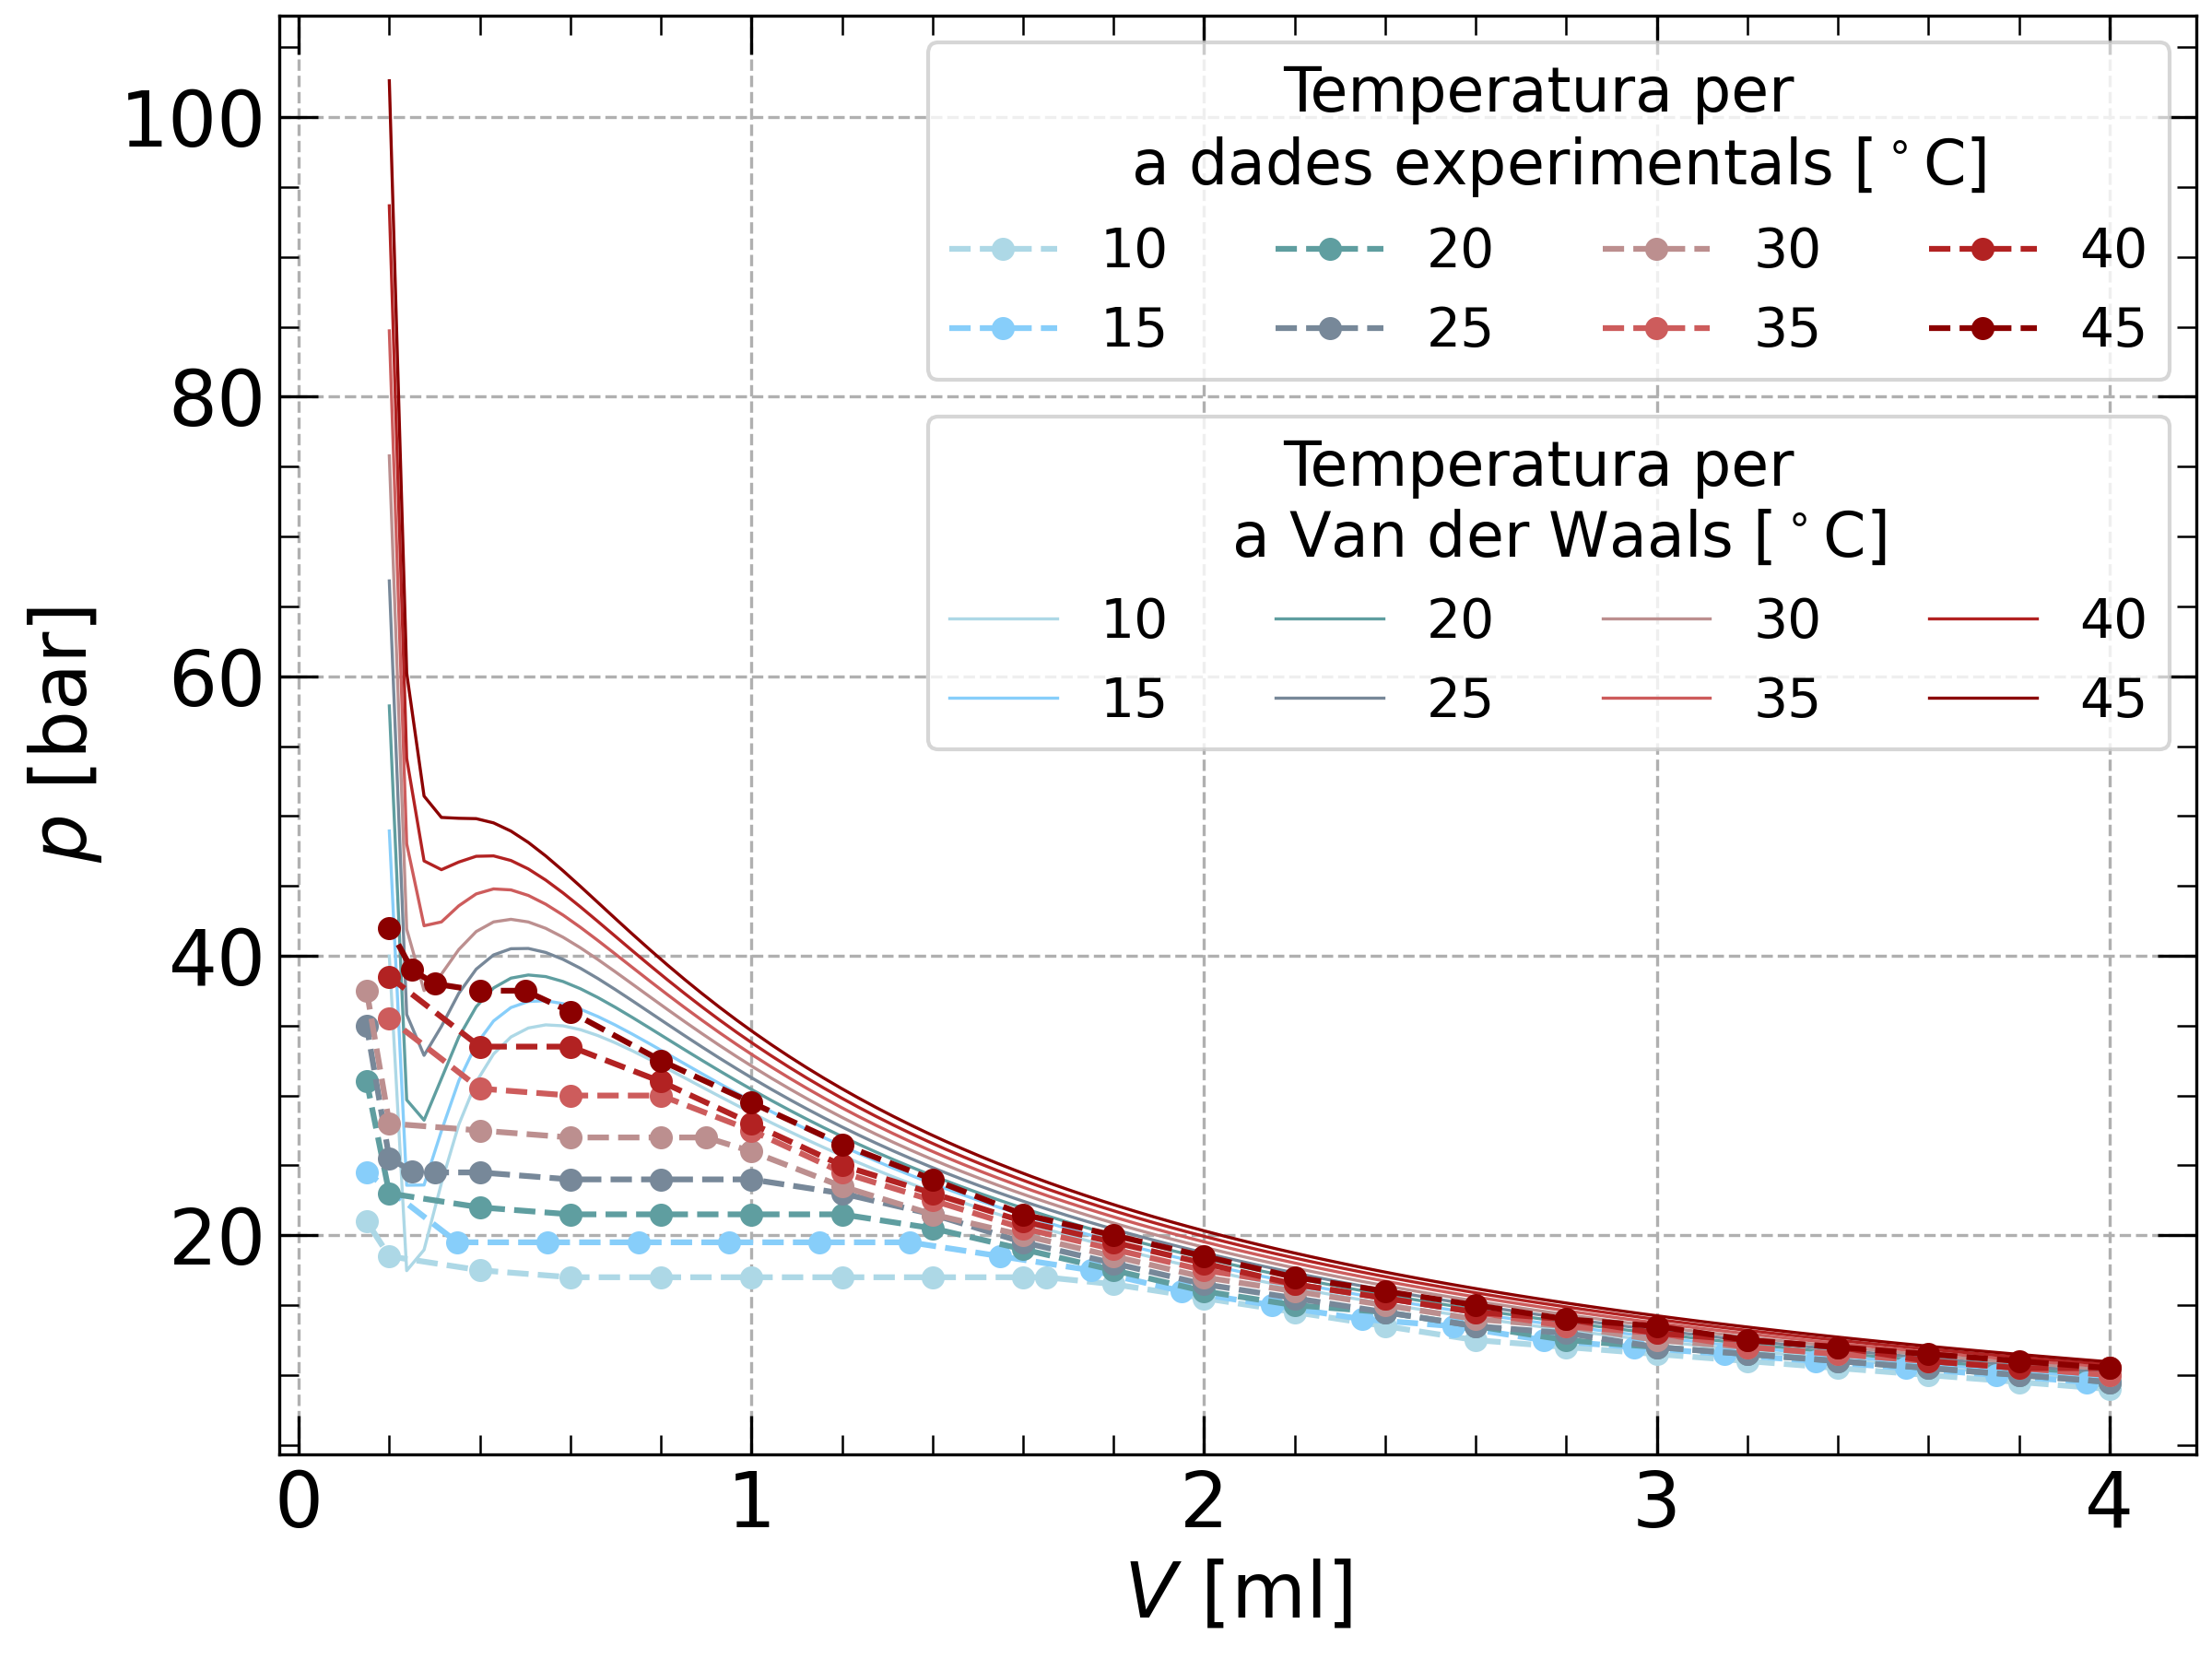
\includegraphics[width=\linewidth]{../../graphs/practica_IIIb/plots/Van_der_Waals_comparativa_completa.png}
  \captionof{figure}{\footnotesize{Comparació de les dades experimentals i les corbes de Van der Waals per a totes les temperatures. Es representen les temperatures amb el mateix degradat de color que la Figura \ref{fig:Diagrama_Clapeyron}.}}
  \label{fig:VdW_vs_exp_complet}
\end{Figura}
\subsection{Tractament de dades de la corba de saturació}
Per tal d'aclarir els canvis concrets entre les dades obtingudes al laboratori i les dades que s'han tingut en compte per a fer els càlculs i representacions de les dades de la corba de saturació, en aquest subapartat de l'Annex es mostren totes les dades a la Taula \ref{tau:comparacio_saturacio}.
\renewcommand{\arraystretch}{1.45}
\begin{Figura}
  \centering
  \captionof{table}{\footnotesize{Comparació de les dades experimentals de la corba de saturació abans i després del tractament. Els valors $p_{\text{m}}$ i $V_{\text{m}}$ són les dades mesurades i $p_{\text{t}}$ i $V_{\text{t}}$ les dades tractades. Les unitats i incertesa de cada magnitud són: $^\circ$C per a la temperatura\protect\footnotemark, \((\pm0,2)\,\text{bar}\) per a la pressió i \((\pm0,05)\,\text{ml}\) per al volum.}}
  \resizebox{\textwidth}{!}{
  \begin{tabular}{c|c|c|c|c}
    \multirow{1}{1cm}{\centering $T$} & \multirow{1}{1.2cm}{\centering $p_{\text{m}}$} & \multirow{1}{1.2cm}{\centering $V_{\text{m}}$} & \multirow{1}{1.2cm}{\centering $p_{\text{t}}$} & \multirow{1}{1.2cm}{\centering $V_{\text{t}}$}  \\
    \hline\hline
    \multirow{2}{*}{10} & 17,0 & 1,65 & 17,0 & 1,65\\[-0.1cm]
                        & 21,0 & 0,15 & 17,0 & 0,15\\[0.3cm]
    \multirow{2}{*}{15} & 19,5 & 1,35 & 19,5 & 1,35\\[-0.1cm]
                        & 24,5 & 0,15 & 19,5 & 0,25\\[0.3cm]
    \multirow{2}{*}{20} & 21,5 & 1,00 & 21,5 & 1,20\\[-0.1cm]
                        & 31,0 & 0,20 & 21,5 & 0,18\\[0.3cm]
    \multirow{2}{*}{25} & 24,0 & 1,00 & 24,0 & 1,10\\[-0.1cm]
                        & 25,5 & 0,20 & 24,0 & 0,20\\[0.3cm]
    \multirow{2}{*}{30} & 27,0 & 0,90 & 27,0 & 0,90\\[-0.1cm]
                        & 37,5 & 0,15 & 27,0 & 0,18\\[0.3cm]
    \multirow{2}{*}{35} & 30,0 & 0,80 & 30,0 & 0,80\\[-0.1cm]
                        & 35,5 & 0,20 & 30,0 & 0,30\\[0.3cm]
    \multirow{2}{*}{40} & 31,0 & 0,80 & 33,5 & 0,70\\[-0.1cm]
                        & 38,5 & 0,20 & 33,5 & 0,30\\[0.3cm]
    \multirow{2}{*}{45} & 37,5 & 0,40 & 37,5 & 0,50\\[-0.1cm]
                        & 39,0 & 0,25 & 37,5 & 0,40\\[0.3cm]
  \end{tabular}
  }
  \label{tau:comparacio_saturacio}
\end{Figura}
\footnotetext{Com s'indica al text principal, aquests valors són les etiquetes i no les mesures de la temperatura, per aquest motiu no s'afegeix incertesa.}
\renewcommand{\arraystretch}{1}
\subsection{Càlcul d'incerteses}
Per a calcular la incertesa dels valors mesurats directament al laboratori s'ha fet servir la desviació estàndard de la mostra obtinguda de cada valor mesurat. Juntament amb la incertesa instrumental, calculem la incertesa de cada mesura com
\begin{equation*}
    u(x_i) = \sqrt{ s_{\text{est}}^2(x_i) + s_{\text{ins}}^2}
\end{equation*}
on $s_{\text{est}}$ és la desviació estàndard, $s_{\text{ins}}$ és la incertesa instrumental i $x_i$ és la variable mesurada.\\\\
Per a calcular la incertesa de magnituds derivades de les variables mesurades, s'ha fet servir la propagació d'incerteses, calculada com
\begin{equation*}
    u^2(y) = \sum_{i = 1}^{n} \left( \frac{\partial y}{\partial{x_i}} u(x_i)\right)^2
\end{equation*}
on $y$ és una funció tal que $y = y(x_1,...,x_n)$.\\\\
Per a calcular els errors de les regressions s'ha fet servir la funció \texttt{curve\_fit} de la llibreria \texttt{scipy.optimize} de Python. Per a calcular els coeficients de regressió $r^2$ s'ha aplicat el mètode de mínims quadrats, també amb Python.
\end{multicols}
\bibliographystyle{plain} 
\bibliography{referencies_IIIb.bib}
\end{document}